% Created 2023-10-26 to 17:38
% Intended LaTeX compiler: pdflatex
\documentclass[12pt]{article}

%%%% settings when exporting code %%%% 

\usepackage{listings}
\lstdefinestyle{code-small}{
backgroundcolor=\color{white}, % background color for the code block
basicstyle=\ttfamily\small, % font used to display the code
commentstyle=\color[rgb]{0.5,0,0.5}, % color used to display comments in the code
keywordstyle=\color{black}, % color used to highlight certain words in the code
numberstyle=\ttfamily\tiny\color{gray}, % color used to display the line numbers
rulecolor=\color{black}, % color of the frame
stringstyle=\color[rgb]{0,.5,0},  % color used to display strings in the code
breakatwhitespace=false, % sets if automatic breaks should only happen at whitespace
breaklines=true, % sets automatic line breaking
columns=fullflexible,
frame=single, % adds a frame around the code (non,leftline,topline,bottomline,lines,single,shadowbox)
keepspaces=true, % % keeps spaces in text, useful for keeping indentation of code
literate={~}{$\sim$}{1}, % symbol properly display via latex
numbers=none, % where to put the line-numbers; possible values are (none, left, right)
numbersep=10pt, % how far the line-numbers are from the code
showspaces=false,
showstringspaces=false,
stepnumber=1, % the step between two line-numbers. If it's 1, each line will be numbered
tabsize=1,
xleftmargin=0cm,
emph={anova,apply,class,coef,colnames,colNames,colSums,dim,dcast,for,ggplot,head,if,ifelse,is.na,lapply,list.files,library,logLik,melt,plot,require,rowSums,sapply,setcolorder,setkey,str,summary,tapply},
aboveskip = \medskipamount, % define the space above displayed listings.
belowskip = \medskipamount, % define the space above displayed listings.
lineskip = 0pt} % specifies additional space between lines in listings
\lstset{style=code-small}
%%%% packages %%%%%

\usepackage[utf8]{inputenc}
\usepackage[T1]{fontenc}
\usepackage{lmodern}
\usepackage{textcomp}
\usepackage{color}
\usepackage{graphicx}
\usepackage{grffile}
\usepackage{wrapfig}
\usepackage{rotating}
\usepackage{longtable}
\usepackage{multirow}
\usepackage{multicol}
\usepackage{changes}
\usepackage{pdflscape}
\usepackage{geometry}
\usepackage[normalem]{ulem}
\usepackage{amssymb}
\usepackage{amsmath}
\usepackage{amsfonts}
\usepackage{dsfont}
\usepackage{array}
\usepackage{ifthen}
\usepackage{hyperref}
\usepackage{natbib}
%
%%%% specifications %%%%
%
\usepackage{ifthen}
\usepackage{xifthen}
\usepackage{xargs}
\usepackage{xspace}
\newcommand\Rlogo{\textbf{\textsf{R}}\xspace} %
\RequirePackage{fancyvrb}
\DefineVerbatimEnvironment{verbatim}{Verbatim}{fontsize=\small,formatcom = {\color[rgb]{0.5,0,0}}}
\RequirePackage{colortbl} % arrayrulecolor to mix colors
\RequirePackage{setspace} % to modify the space between lines - incompatible with footnote in beamer
\renewcommand{\baselinestretch}{1.1}
\geometry{top=2cm,bottom=3cm,left=1.5cm,right=1.5cm}
\RequirePackage{changepage}
\RequirePackage{colortbl} % arrayrulecolor to mix colors
\RequirePackage{pifont}
\RequirePackage{relsize}
\newcommand{\Cross}{{\raisebox{-0.5ex}%
{\relsize{1.5}\ding{56}}}\hspace{1pt} }
\newcommand{\Valid}{{\raisebox{-0.5ex}%
{\relsize{1.5}\ding{52}}}\hspace{1pt} }
\newcommand{\CrossR}{ \textcolor{red}{\Cross} }
\newcommand{\ValidV}{ \textcolor{green}{\Valid} }
\usepackage{stackengine}
\usepackage{scalerel}
\newcommand\Warning[1][3ex]{%
\renewcommand\stacktype{L}%
\scaleto{\stackon[1.3pt]{\color{red}$\triangle$}{\tiny\bfseries !}}{#1}%
\xspace
}
\hypersetup{
citecolor=[rgb]{0,0.5,0},
urlcolor=[rgb]{0,0,0.5},
linkcolor=[rgb]{0,0,0.5},
}
\RequirePackage{epstopdf} % to be able to convert .eps to .pdf image files
\RequirePackage{capt-of} %
\RequirePackage{caption} % newlines in graphics
\RequirePackage{enumitem} % to be able to convert .eps to .pdf image files
\definecolor{light}{rgb}{1, 1, 0.9}
\definecolor{lightred}{rgb}{1.0, 0.7, 0.7}
\definecolor{lightblue}{rgb}{0.0, 0.8, 0.8}
\newcommand{\darkblue}{blue!80!black}
\newcommand{\darkgreen}{green!50!black}
\newcommand{\darkred}{red!50!black}
\usepackage{mdframed}
\newcommand{\first}{1\textsuperscript{st} }
\newcommand{\second}{2\textsuperscript{nd} }
\newcommand{\third}{3\textsuperscript{rd} }
\date{\today}
\title{Results simulation study DelayedGSD}
\hypersetup{
 colorlinks=true,
 pdfauthor={},
 pdftitle={Results simulation study DelayedGSD},
 pdfkeywords={},
 pdfsubject={},
 pdfcreator={Emacs 27.2 (Org mode 9.5.2)},
 pdflang={English}
 }
\begin{document}

\maketitle

\section{Rejection rate}
\label{sec:org447cb16}

\subsection{2 stages}
\label{sec:org55b74fa}
Power by method (columns) and scenario (rows): \hfill (nominal level 80\%)
\begin{verbatim}
 scenario n.sim missing binding  fixC ar method 1 method 2 method 3
        1 10000    TRUE    TRUE FALSE 10   81.00%   80.93%   80.43%
        3 10000    TRUE    TRUE FALSE  5   80.53%   80.53%   80.14%
        5 10000    TRUE    TRUE  TRUE 10   80.15%   80.35%   80.43%
        7 10000    TRUE    TRUE  TRUE  5   80.08%   80.20%   80.14%
        9 10000    TRUE   FALSE  TRUE 10   79.86%   80.12%   80.26%
       11 10000    TRUE   FALSE  TRUE  5   79.93%   80.04%   80.06%
       13 10000    TRUE   FALSE FALSE 10   80.50%   80.44%   80.26%
       15 10000    TRUE   FALSE FALSE  5   80.37%   80.36%   80.06%
       17 10000   FALSE    TRUE FALSE  5   80.31%   80.30%   79.92%
\end{verbatim}

\bigskip

Type 1 error by method (columns) and scenario (rows): \hfill (nominal level 2.5\%)
\begin{verbatim}
 scenario n.sim missing binding  fixC ar method 1 method 2 method 3
        2 10000    TRUE    TRUE FALSE 10    2.42%    2.39%    2.37%
        4 10000    TRUE    TRUE FALSE  5    2.40%    2.40%    2.35%
        6 10000    TRUE    TRUE  TRUE 10    2.24%    2.22%    2.37%
        8 10000    TRUE    TRUE  TRUE  5    2.32%    2.31%    2.35%
       10 10000    TRUE   FALSE  TRUE 10    2.45%    2.47%    2.57%
       12 10000    TRUE   FALSE  TRUE  5    2.63%    2.64%    2.66%
       14 10000    TRUE   FALSE FALSE 10    2.53%    2.53%    2.57%
       16 10000    TRUE   FALSE FALSE  5    2.68%    2.68%    2.66%
       18 10000   FALSE    TRUE FALSE  5    2.46%    2.46%    2.45%
\end{verbatim}

\clearpage

\begin{figure}[!h]
\centering
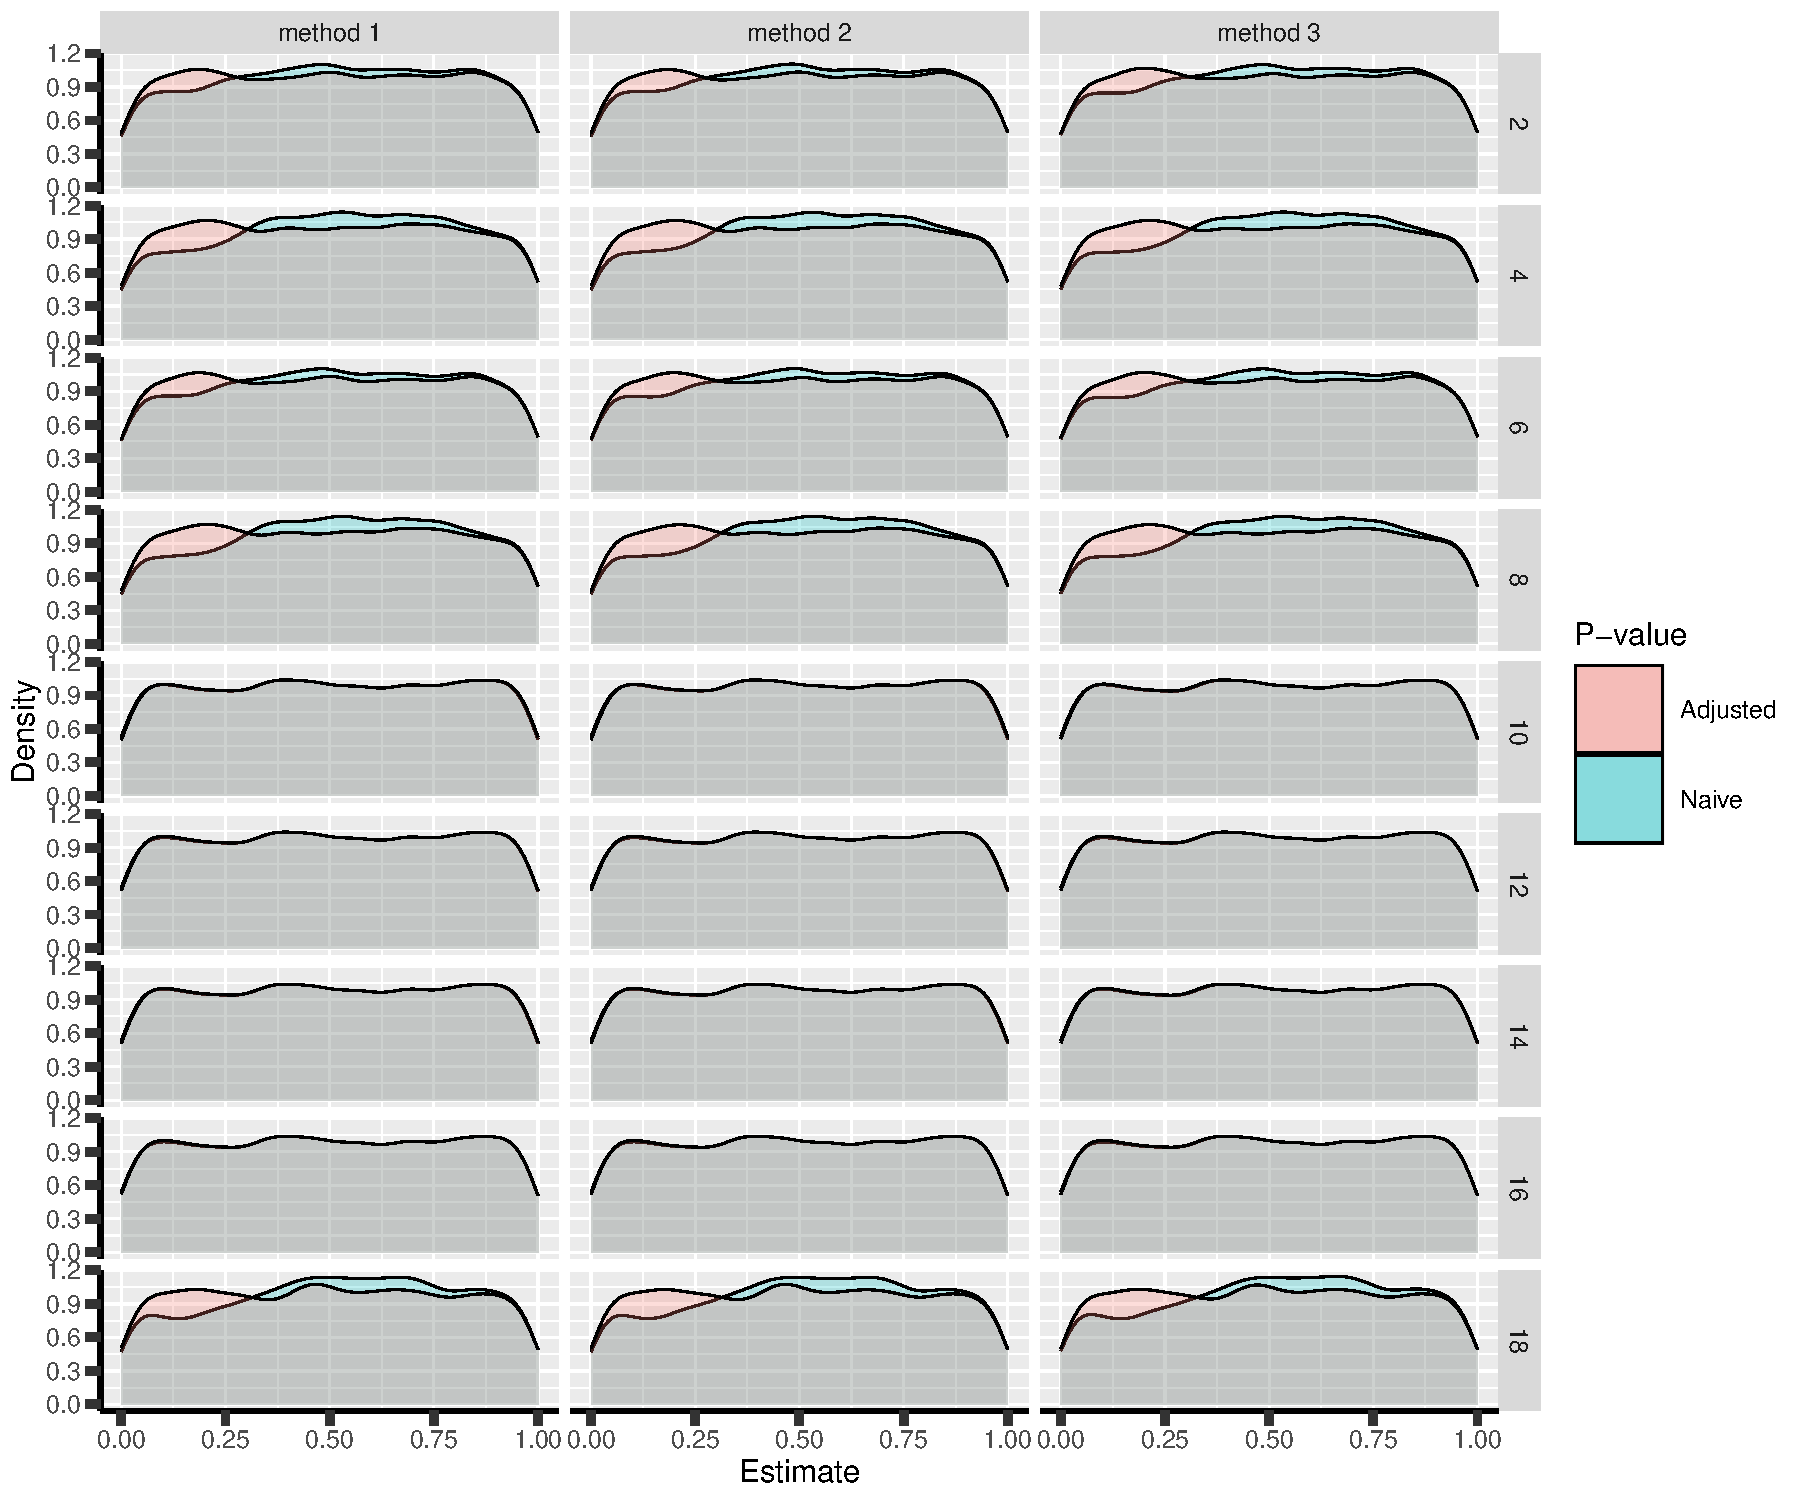
\includegraphics[trim={0 0 0 0},width=1\textwidth]{./figures/gg2stage-pvalue-density.pdf}
\caption{Naive and adjusted p-value distribution over all simulations under the null. Each row correspond to a different scenario}
\end{figure}

\begin{figure}[!h]
\centering
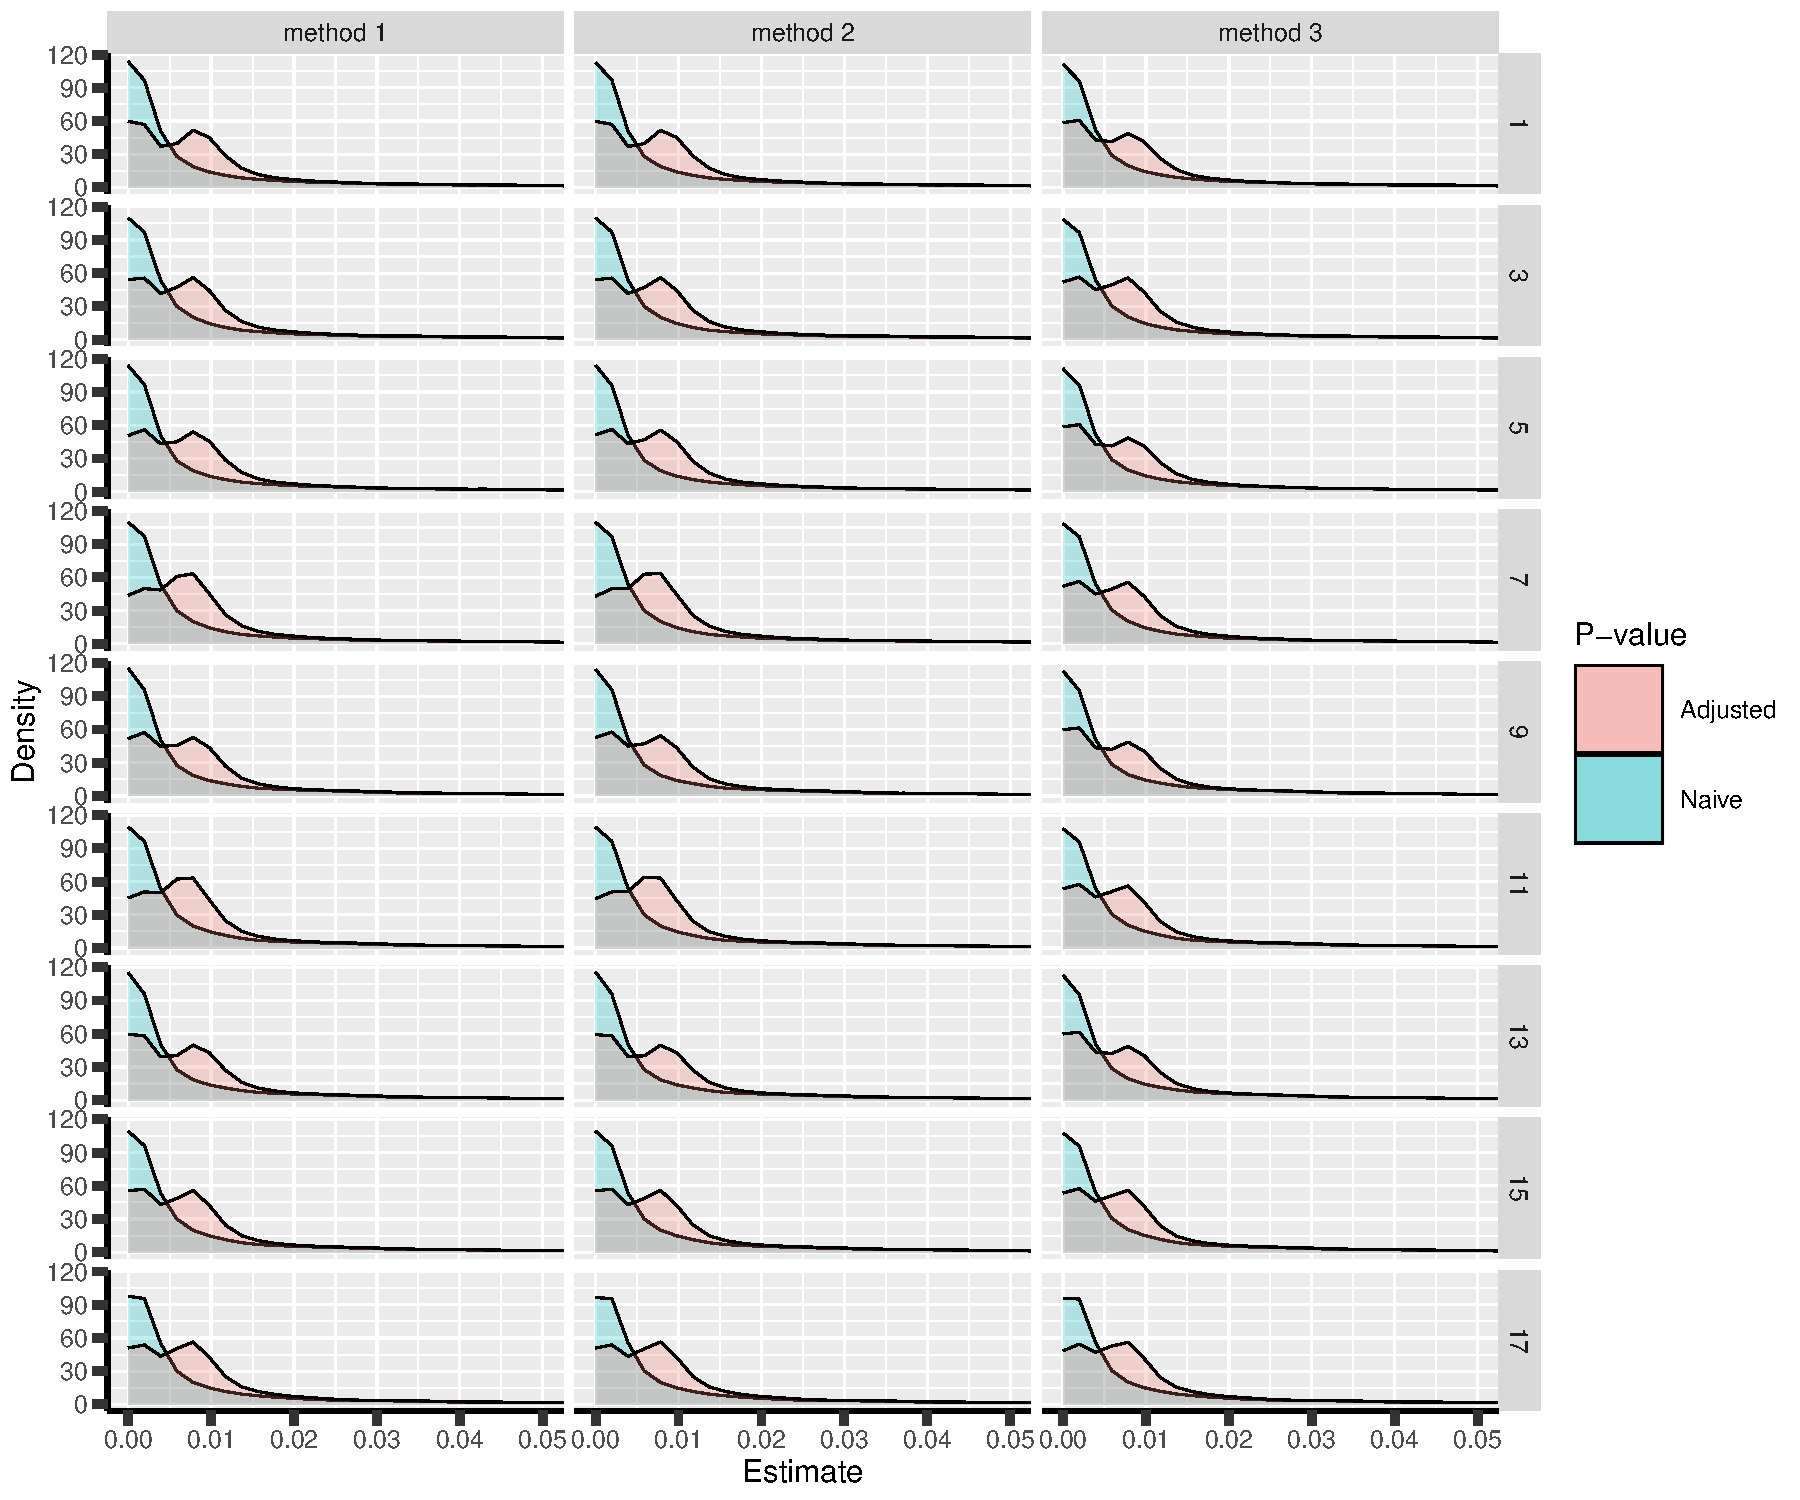
\includegraphics[trim={0 0 0 0},width=1\textwidth]{./figures/gg2stage-pvalue2-density.pdf}
\caption{Naive and adjusted p-value distribution over all simulations under the alternative. Each row correspond to a different scenario}
\end{figure}

\clearpage

\subsection{3 stages}
\label{sec:org1223c05}

Power by method (columns) and scenario (rows): \hfill (nominal level 80\%)
\begin{verbatim}
 scenario n.sim missing binding  fixC ar method 1 method 2 method 3
        1 10000    TRUE    TRUE FALSE 10   80.87%   80.79%   80.14%
        3  9921    TRUE    TRUE FALSE  5   80.57%   80.56%   80.08%
        5 10000    TRUE    TRUE  TRUE 10   79.84%   80.05%   80.14%
        7  9921    TRUE    TRUE  TRUE  5   79.98%   80.08%   80.08%
        9 10000    TRUE   FALSE  TRUE 10   79.58%   79.94%   80.06%
       11 10000    TRUE   FALSE  TRUE  5   79.92%   80.15%   79.96%
       13 10000    TRUE   FALSE FALSE 10   80.52%   80.44%   80.06%
       15 10000    TRUE   FALSE FALSE  5   80.44%   80.42%   79.96%
       17 10000   FALSE    TRUE FALSE  5   80.23%   80.21%   79.80%
\end{verbatim}

\bigskip

Type 1 error by method (columns) and scenario (rows): \hfill (nominal level 2.5\%)
\begin{verbatim}
 scenario n.sim missing binding  fixC ar method 1 method 2 method 3
        2 10000    TRUE    TRUE FALSE 10    2.50%    2.48%    2.38%
        4 10000    TRUE    TRUE FALSE  5    2.42%    2.43%    2.40%
        6 10000    TRUE    TRUE  TRUE 10    2.31%    2.33%    2.38%
        8 10000    TRUE    TRUE  TRUE  5    2.37%    2.36%    2.40%
       10 10000    TRUE   FALSE  TRUE 10    2.44%    2.42%    2.52%
       12 10000    TRUE   FALSE  TRUE  5    2.48%    2.48%    2.54%
       14 10000    TRUE   FALSE FALSE 10    2.54%    2.53%    2.52%
       16 10000    TRUE   FALSE FALSE  5    2.61%    2.61%    2.54%
       18 10000   FALSE    TRUE FALSE  5    2.57%    2.57%    2.48%
\end{verbatim}

\clearpage

\begin{figure}[!h]
\centering
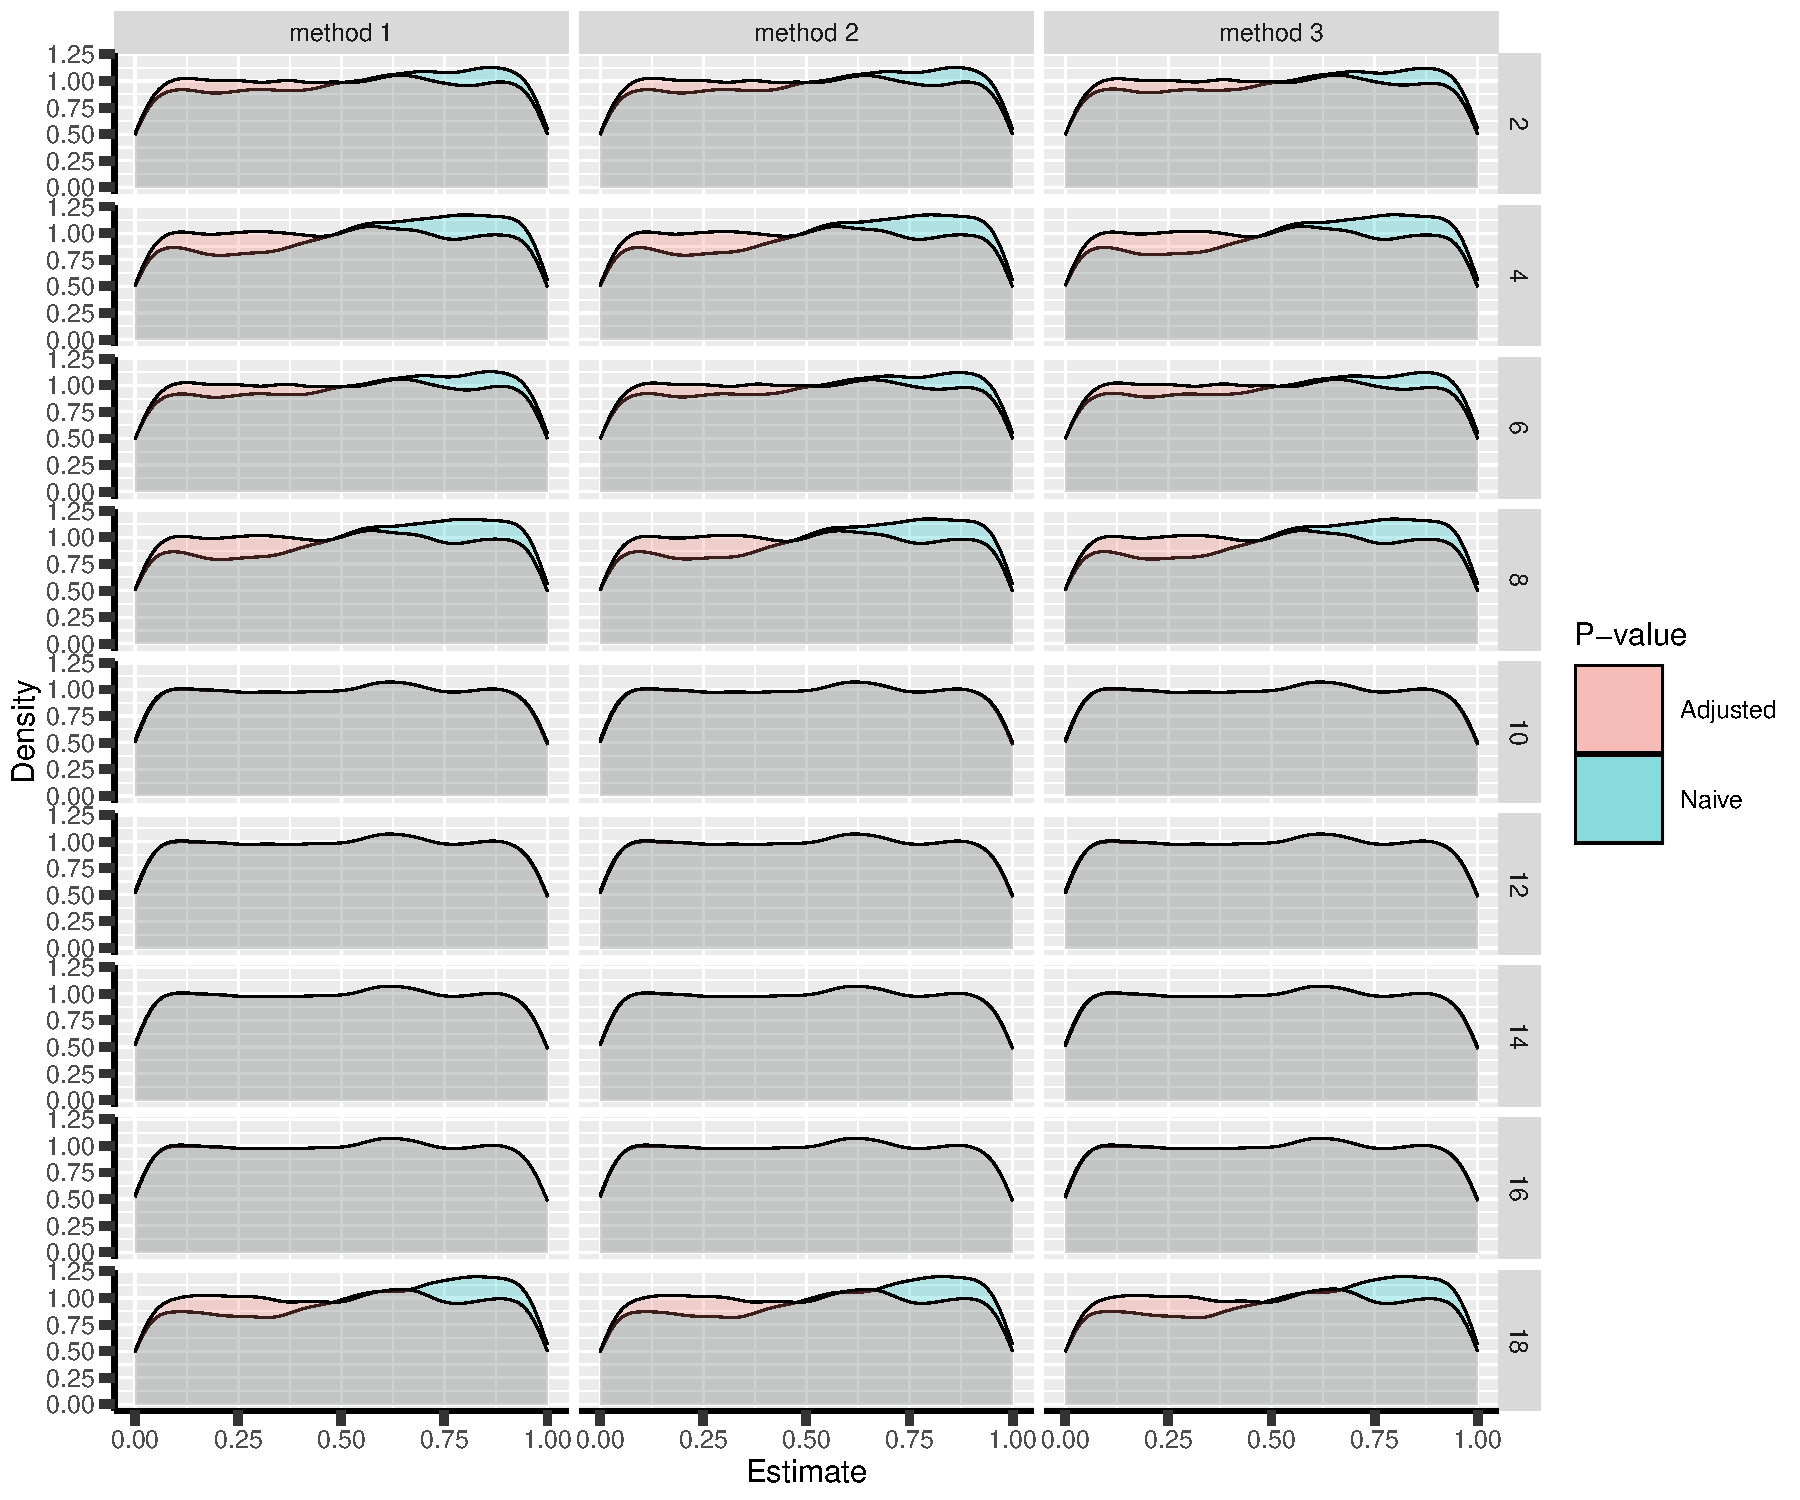
\includegraphics[trim={0 0 0 0},width=1\textwidth]{./figures/gg3stage-pvalue-density.pdf}
\caption{Naive and adjusted p-value distribution over all simulations under the null. Each row correspond to a different scenario}
\end{figure}

\begin{figure}[!h]
\centering
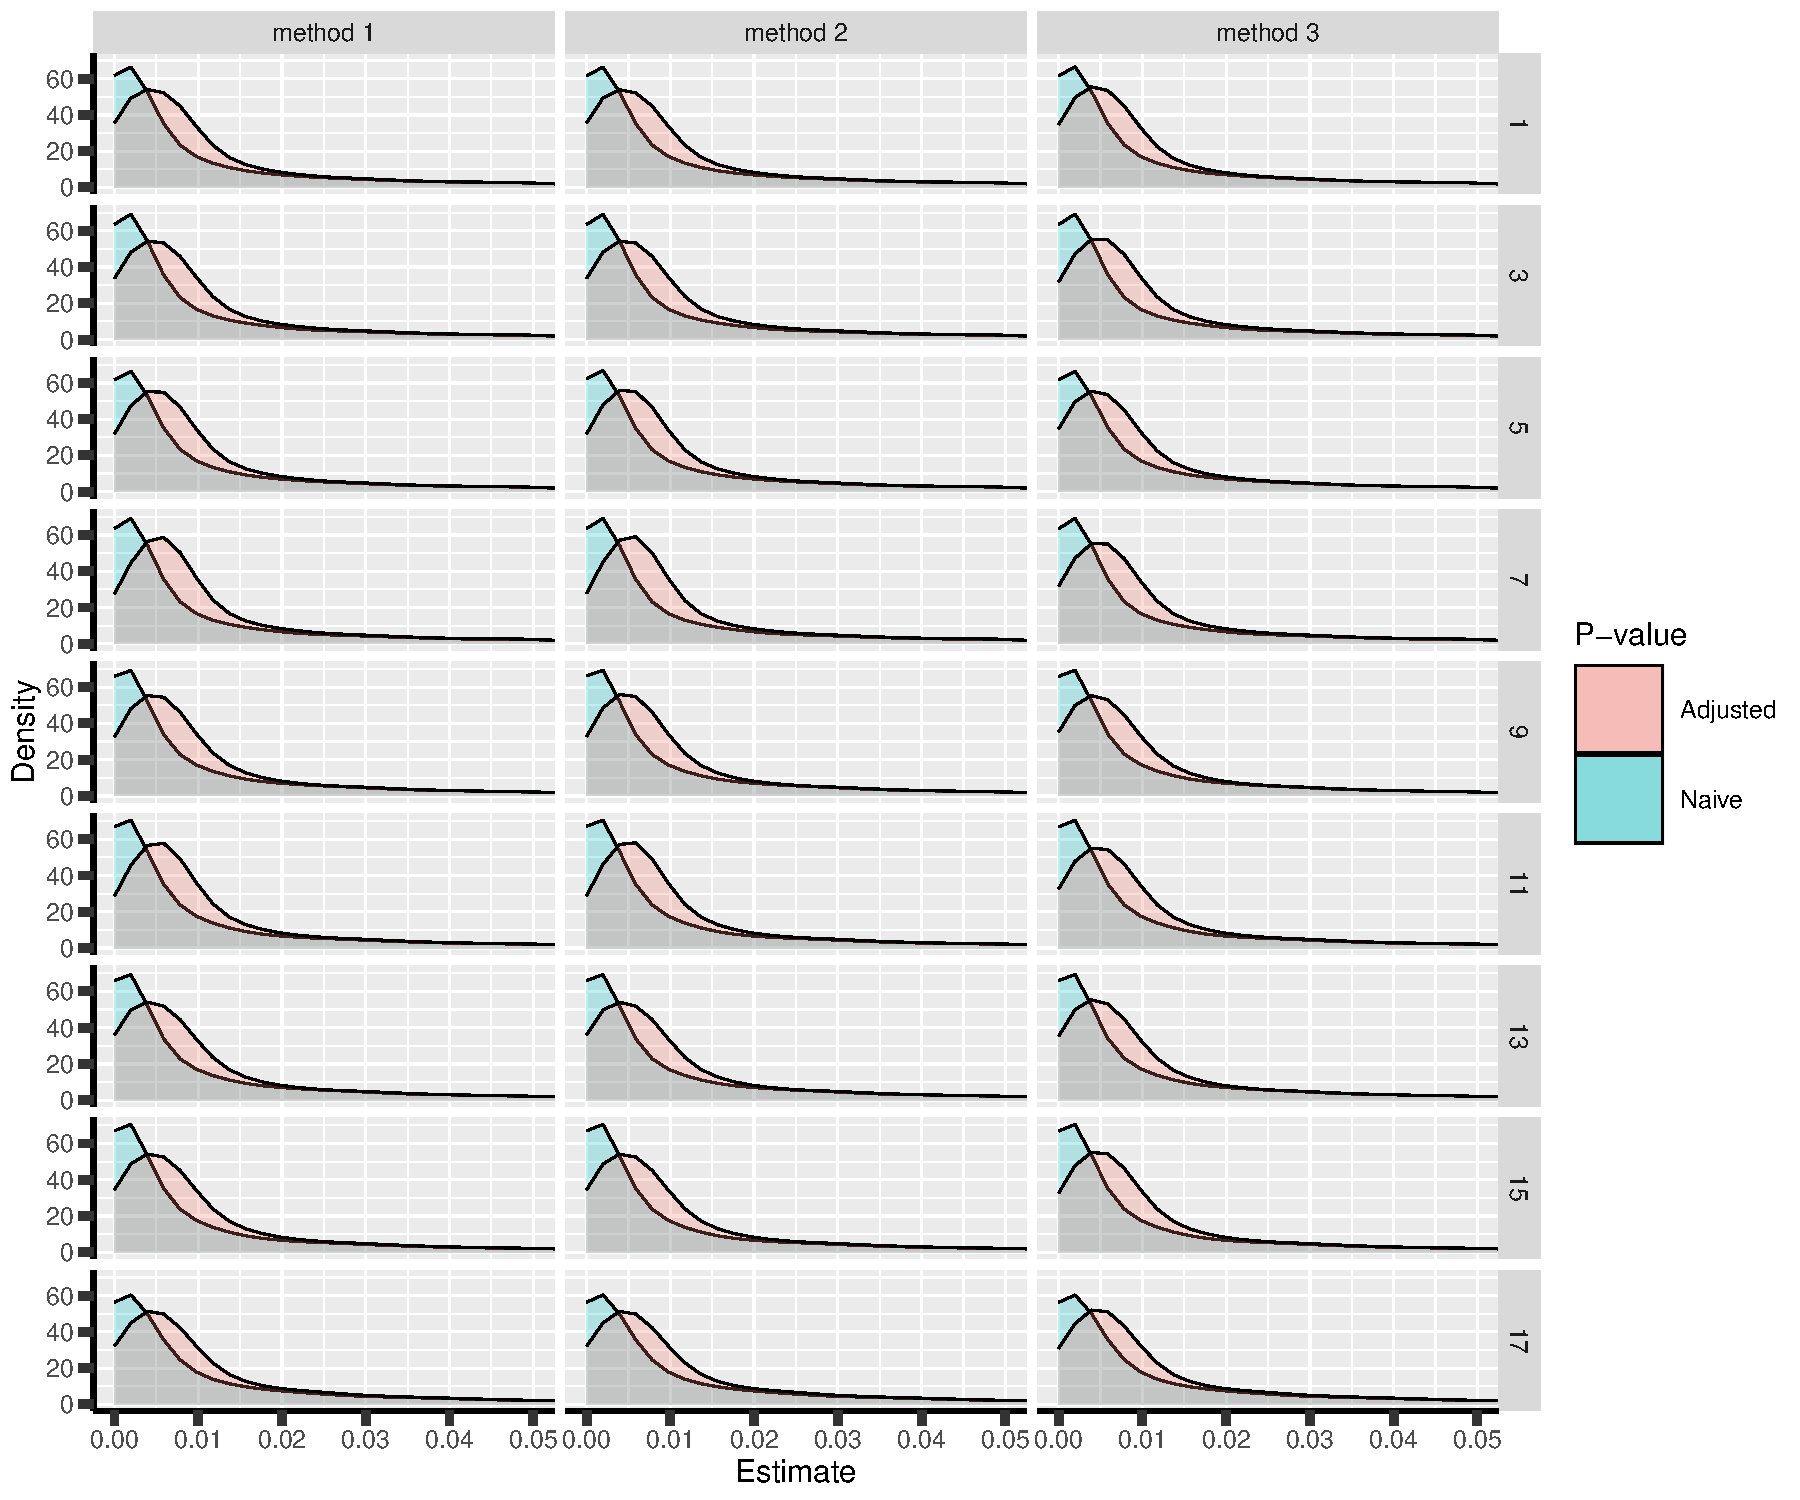
\includegraphics[trim={0 0 0 0},width=1\textwidth]{./figures/gg-pvalue2-density.pdf}
\caption{Naive and adjusted p-value distribution over all simulations under the alternative. Each row correspond to a different scenario}
\end{figure}

\clearpage

\section{Conclusion of the trial}
\label{sec:org22a2285}

\subsection{2 stages}
\label{sec:org13fae18}
Relative frequency of stopping for efficacy/futility at decision/final

\begin{itemize}
\item Method 1
\end{itemize}
\begin{verbatim}
        N missing  hypo binding  fixC ar decision.eff decision.fut final.eff final.fut
 1: 10000    TRUE power    TRUE FALSE 10       37.79%        5.93%    43.21%    13.07%
 2: 10000    TRUE typeI    TRUE FALSE 10        0.80%       71.13%     1.62%    26.45%
 3: 10000    TRUE power    TRUE FALSE  5       35.74%        5.98%    44.79%    13.49%
 4: 10000    TRUE typeI    TRUE FALSE  5        0.74%       69.32%     1.66%    28.28%
 5: 10000    TRUE power    TRUE  TRUE 10       36.94%        6.78%    43.21%    13.07%
 6: 10000    TRUE typeI    TRUE  TRUE 10        0.62%       71.31%     1.62%    26.45%
 7: 10000    TRUE power    TRUE  TRUE  5       35.29%        6.43%    44.79%    13.49%
 8: 10000    TRUE typeI    TRUE  TRUE  5        0.66%       69.40%     1.66%    28.28%
 9: 10000    TRUE power   FALSE  TRUE 10       38.05%        6.57%    41.81%    13.57%
10: 10000    TRUE typeI   FALSE  TRUE 10        0.61%        0.20%     1.84%    97.35%
11: 10000    TRUE power   FALSE  TRUE  5       36.35%        6.15%    43.58%    13.92%
12: 10000    TRUE typeI   FALSE  TRUE  5        0.70%        0.06%     1.93%    97.31%
13: 10000    TRUE power   FALSE FALSE 10       38.69%        5.93%    41.81%    13.57%
14: 10000    TRUE typeI   FALSE FALSE 10        0.69%        0.12%     1.84%    97.35%
15: 10000    TRUE power   FALSE FALSE  5       36.79%        5.71%    43.58%    13.92%
16: 10000    TRUE typeI   FALSE FALSE  5        0.75%        0.01%     1.93%    97.31%
17: 10000   FALSE power    TRUE FALSE  5       33.98%        5.33%    46.33%    14.36%
18: 10000   FALSE typeI    TRUE FALSE  5        0.74%       67.48%     1.72%    30.06%
\end{verbatim}

\clearpage

Method 2:
\begin{verbatim}
        N missing  hypo binding  fixC ar decision.eff decision.fut final.eff final.fut
 1: 10000    TRUE power    TRUE FALSE 10       37.85%        6.19%    43.08%    12.88%
 2: 10000    TRUE typeI    TRUE FALSE 10        0.79%       71.64%     1.60%    25.97%
 3: 10000    TRUE power    TRUE FALSE  5       35.77%        5.99%    44.76%    13.48%
 4: 10000    TRUE typeI    TRUE FALSE  5        0.74%       69.38%     1.66%    28.22%
 5: 10000    TRUE power    TRUE  TRUE 10       36.69%        6.24%    43.66%    13.41%
 6: 10000    TRUE typeI    TRUE  TRUE 10        0.59%       69.61%     1.63%    28.17%
 7: 10000    TRUE power    TRUE  TRUE  5       35.02%        6.05%    45.18%    13.75%
 8: 10000    TRUE typeI    TRUE  TRUE  5        0.63%       68.36%     1.68%    29.33%
 9: 10000    TRUE power   FALSE  TRUE 10       37.85%        6.04%    42.27%    13.84%
10: 10000    TRUE typeI   FALSE  TRUE 10        0.61%        0.19%     1.86%    97.34%
11: 10000    TRUE power   FALSE  TRUE  5       36.18%        5.84%    43.86%    14.12%
12: 10000    TRUE typeI   FALSE  TRUE  5        0.69%        0.06%     1.95%    97.30%
13: 10000    TRUE power   FALSE FALSE 10       38.70%        6.09%    41.74%    13.47%
14: 10000    TRUE typeI   FALSE FALSE 10        0.69%        0.12%     1.84%    97.35%
15: 10000    TRUE power   FALSE FALSE  5       36.82%        5.75%    43.54%    13.89%
16: 10000    TRUE typeI   FALSE FALSE  5        0.75%        0.01%     1.93%    97.31%
17: 10000   FALSE power    TRUE FALSE  5       34.03%        5.36%    46.27%    14.34%
18: 10000   FALSE typeI    TRUE FALSE  5        0.74%       67.55%     1.72%    29.99%
\end{verbatim}

Method 3:
\begin{verbatim}
        N missing  hypo binding  fixC ar decision.eff decision.fut final.eff final.fut
 1: 10000    TRUE power    TRUE FALSE 10       40.58%        6.53%    39.85%    13.04%
 2: 10000    TRUE typeI    TRUE FALSE 10        0.74%       68.79%     1.63%    28.84%
 3: 10000    TRUE power    TRUE FALSE  5       36.54%        6.30%    43.60%    13.56%
 4: 10000    TRUE typeI    TRUE FALSE  5        0.69%       68.41%     1.66%    29.24%
 5: 10000    TRUE power    TRUE  TRUE 10       40.58%        6.53%    39.85%    13.04%
 6: 10000    TRUE typeI    TRUE  TRUE 10        0.74%       68.79%     1.63%    28.84%
 7: 10000    TRUE power    TRUE  TRUE  5       36.54%        6.30%    43.60%    13.56%
 8: 10000    TRUE typeI    TRUE  TRUE  5        0.69%       68.41%     1.66%    29.24%
 9: 10000    TRUE power   FALSE  TRUE 10       41.34%        6.20%    38.92%    13.54%
10: 10000    TRUE typeI   FALSE  TRUE 10        0.77%        0.33%     1.80%    97.10%
11: 10000    TRUE power   FALSE  TRUE  5       37.71%        6.03%    42.35%    13.91%
12: 10000    TRUE typeI   FALSE  TRUE  5        0.73%        0.09%     1.93%    97.25%
13: 10000    TRUE power   FALSE FALSE 10       41.34%        6.20%    38.92%    13.54%
14: 10000    TRUE typeI   FALSE FALSE 10        0.77%        0.33%     1.80%    97.10%
15: 10000    TRUE power   FALSE FALSE  5       37.71%        6.03%    42.35%    13.91%
16: 10000    TRUE typeI   FALSE FALSE  5        0.73%        0.09%     1.93%    97.25%
17: 10000   FALSE power    TRUE FALSE  5       34.65%        5.59%    45.27%    14.49%
18: 10000   FALSE typeI    TRUE FALSE  5        0.68%       66.54%     1.77%    31.01%
\end{verbatim}

\clearpage

Relative frequency of stopping for with a threshold below 1.96:
\begin{verbatim}
    scenario missing method binding  fixC ar  hypo     N rejection rejectionBelow196
 1:        1    TRUE      1    TRUE FALSE 10 power 10000    81.00%             0.85%
 2:        1    TRUE      2    TRUE FALSE 10 power 10000    80.93%             0.84%
 3:        2    TRUE      1    TRUE FALSE 10 typeI 10000     2.42%             0.18%
 4:        2    TRUE      2    TRUE FALSE 10 typeI 10000     2.39%             0.17%
 5:        3    TRUE      1    TRUE FALSE  5 power 10000    80.53%             0.45%
 6:        3    TRUE      2    TRUE FALSE  5 power 10000    80.53%             0.45%
 7:        4    TRUE      1    TRUE FALSE  5 typeI 10000     2.40%             0.08%
 8:        4    TRUE      2    TRUE FALSE  5 typeI 10000     2.40%             0.08%
 9:       13    TRUE      1   FALSE FALSE 10 power 10000    80.50%             0.64%
10:       13    TRUE      2   FALSE FALSE 10 power 10000    80.44%             0.64%
11:       14    TRUE      1   FALSE FALSE 10 typeI 10000     2.53%             0.08%
12:       14    TRUE      2   FALSE FALSE 10 typeI 10000     2.53%             0.08%
13:       15    TRUE      1   FALSE FALSE  5 power 10000    80.37%             0.44%
14:       15    TRUE      2   FALSE FALSE  5 power 10000    80.36%             0.44%
15:       16    TRUE      1   FALSE FALSE  5 typeI 10000     2.68%             0.05%
16:       16    TRUE      2   FALSE FALSE  5 typeI 10000     2.68%             0.05%
17:       17   FALSE      1    TRUE FALSE  5 power 10000    80.31%             0.42%
18:       17   FALSE      2    TRUE FALSE  5 power 10000    80.30%             0.43%
19:       18   FALSE      1    TRUE FALSE  5 typeI 10000     2.46%             0.08%
20:       18   FALSE      2    TRUE FALSE  5 typeI 10000     2.46%             0.08%
\end{verbatim}

\clearpage

\subsection{3 stages}
\label{sec:orgb33adc8}
Relative frequency of stopping for efficacy/futility at decision/final

\begin{itemize}
\item Method 1
\end{itemize}
\begin{verbatim}
        N missing  hypo binding  fixC ar dec1.eff dec1.fut dec2.eff dec2.fut final.eff final.fut
 1: 10000    TRUE power    TRUE FALSE 10   19.91%    2.95%   29.31%    5.36%    31.65%    10.82%
 2: 10000    TRUE typeI    TRUE FALSE 10    0.38%   46.24%    0.67%   35.38%     1.45%    15.88%
 3:  9921    TRUE power    TRUE FALSE  5   18.33%    2.79%   28.75%    5.42%    33.48%    11.22%
 4: 10000    TRUE typeI    TRUE FALSE  5    0.36%   44.03%    0.59%   36.50%     1.47%    17.05%
 5: 10000    TRUE power    TRUE  TRUE 10   19.39%    3.47%   28.80%    5.87%    31.65%    10.82%
 6: 10000    TRUE typeI    TRUE  TRUE 10    0.30%   46.32%    0.56%   35.49%     1.45%    15.88%
 7:  9921    TRUE power    TRUE  TRUE  5   18.07%    3.05%   28.42%    5.75%    33.48%    11.22%
 8: 10000    TRUE typeI    TRUE  TRUE  5    0.34%   44.05%    0.56%   36.53%     1.47%    17.05%
 9: 10000    TRUE power   FALSE  TRUE 10   20.80%    3.52%   27.86%    5.59%    30.92%    11.31%
10: 10000    TRUE typeI   FALSE  TRUE 10    0.31%    0.10%    0.51%    0.63%     1.62%    96.83%
11: 10000    TRUE power   FALSE  TRUE  5   19.31%    3.03%   28.11%    5.68%    32.50%    11.37%
12: 10000    TRUE typeI   FALSE  TRUE  5    0.31%    0.04%    0.52%    0.10%     1.65%    97.38%
13: 10000    TRUE power   FALSE FALSE 10   21.28%    3.04%   28.32%    5.13%    30.92%    11.31%
14: 10000    TRUE typeI   FALSE FALSE 10    0.35%    0.06%    0.57%    0.57%     1.62%    96.83%
15: 10000    TRUE power   FALSE FALSE  5   19.50%    2.84%   28.44%    5.35%    32.50%    11.37%
16: 10000    TRUE typeI   FALSE FALSE  5    0.35%        0    0.61%    0.01%     1.65%    97.38%
17: 10000   FALSE power    TRUE FALSE  5   17.63%    2.93%   28.90%    5.11%    33.70%    11.73%
18: 10000   FALSE typeI    TRUE FALSE  5    0.48%   42.39%    0.71%   36.38%     1.38%    18.66%
\end{verbatim}

\begin{itemize}
\item Method 2
\end{itemize}
\begin{verbatim}
        N missing  hypo binding  fixC ar dec1.eff dec1.fut dec2.eff dec2.fut final.eff final.fut
 1: 10000    TRUE power    TRUE FALSE 10   19.94%    2.99%   29.32%    5.69%    31.53%    10.53%
 2: 10000    TRUE typeI    TRUE FALSE 10    0.38%   46.48%    0.66%   35.66%     1.44%    15.38%
 3:  9921    TRUE power    TRUE FALSE  5   18.34%    2.82%   28.81%    5.44%    33.40%    11.18%
 4: 10000    TRUE typeI    TRUE FALSE  5    0.36%   44.08%    0.59%   36.47%     1.48%    17.02%
 5: 10000    TRUE power    TRUE  TRUE 10   19.17%    3.16%   28.74%    5.67%    32.14%    11.12%
 6: 10000    TRUE typeI    TRUE  TRUE 10    0.29%   44.63%    0.56%   36.01%     1.48%    17.03%
 7:  9921    TRUE power    TRUE  TRUE  5   17.92%    2.97%   28.25%    5.36%    33.91%    11.58%
 8: 10000    TRUE typeI    TRUE  TRUE  5    0.34%   43.09%    0.54%   36.68%     1.48%    17.87%
 9: 10000    TRUE power   FALSE  TRUE 10   20.72%    3.21%   27.71%    5.29%    31.51%    11.56%
10: 10000    TRUE typeI   FALSE  TRUE 10    0.29%    0.10%    0.50%    0.49%     1.63%    96.99%
11: 10000    TRUE power   FALSE  TRUE  5   19.19%    2.94%   28.01%    5.23%    32.95%    11.68%
12: 10000    TRUE typeI   FALSE  TRUE  5    0.31%    0.04%    0.50%    0.09%     1.67%    97.39%
13: 10000    TRUE power   FALSE FALSE 10   21.30%    3.09%   28.33%    5.27%    30.81%    11.20%
14: 10000    TRUE typeI   FALSE FALSE 10    0.35%    0.06%    0.57%    0.58%     1.61%    96.83%
15: 10000    TRUE power   FALSE FALSE  5   19.51%    2.84%   28.44%    5.39%    32.47%    11.35%
16: 10000    TRUE typeI   FALSE FALSE  5    0.35%        0    0.61%    0.01%     1.65%    97.38%
17: 10000   FALSE power    TRUE FALSE  5   17.68%    2.94%   28.89%    5.17%    33.64%    11.68%
18: 10000   FALSE typeI    TRUE FALSE  5    0.48%   42.46%    0.71%   36.41%     1.38%    18.56%
\end{verbatim}

\clearpage

\begin{itemize}
\item Method 3
\end{itemize}
\begin{verbatim}
        N missing  hypo binding  fixC ar dec1.eff dec1.fut dec2.eff dec2.fut final.eff final.fut
 1: 10000    TRUE power    TRUE FALSE 10   21.49%    3.26%   29.79%    5.96%    28.86%    10.64%
 2: 10000    TRUE typeI    TRUE FALSE 10    0.32%   44.14%    0.60%   35.96%     1.46%    17.52%
 3:  9921    TRUE power    TRUE FALSE  5   18.55%    3.10%   28.93%    5.47%    32.61%    11.34%
 4: 10000    TRUE typeI    TRUE FALSE  5    0.37%   43.25%    0.56%   36.60%     1.47%    17.75%
 5: 10000    TRUE power    TRUE  TRUE 10   21.49%    3.26%   29.79%    5.96%    28.86%    10.64%
 6: 10000    TRUE typeI    TRUE  TRUE 10    0.32%   44.14%    0.60%   35.96%     1.46%    17.52%
 7:  9921    TRUE power    TRUE  TRUE  5   18.55%    3.10%   28.93%    5.47%    32.61%    11.34%
 8: 10000    TRUE typeI    TRUE  TRUE  5    0.37%   43.25%    0.56%   36.60%     1.47%    17.75%
 9: 10000    TRUE power   FALSE  TRUE 10   22.78%    3.32%   28.92%    5.74%    28.36%    10.88%
10: 10000    TRUE typeI   FALSE  TRUE 10    0.33%    0.14%    0.65%    0.81%     1.54%    96.53%
11: 10000    TRUE power   FALSE  TRUE  5   19.70%    3.12%   28.62%    5.49%    31.64%    11.43%
12: 10000    TRUE typeI   FALSE  TRUE  5    0.32%    0.06%    0.59%    0.13%     1.63%    97.27%
13: 10000    TRUE power   FALSE FALSE 10   22.78%    3.32%   28.92%    5.74%    28.36%    10.88%
14: 10000    TRUE typeI   FALSE FALSE 10    0.33%    0.14%    0.65%    0.81%     1.54%    96.53%
15: 10000    TRUE power   FALSE FALSE  5   19.70%    3.12%   28.62%    5.49%    31.64%    11.43%
16: 10000    TRUE typeI   FALSE FALSE  5    0.32%    0.06%    0.59%    0.13%     1.63%    97.27%
17: 10000   FALSE power    TRUE FALSE  5   18.08%    3.12%   29.02%    5.26%    32.70%    11.82%
18: 10000   FALSE typeI    TRUE FALSE  5    0.41%   41.65%    0.68%   36.42%     1.39%    19.45%
\end{verbatim}

Relative frequency of stopping for with a threshold below 1.96:
\begin{verbatim}
    scenario missing method binding  fixC ar  hypo     N rejection rejectionBelow196
 1:        1    TRUE      1    TRUE FALSE 10 power 10000    80.87%             1.03%
 2:        1    TRUE      2    TRUE FALSE 10 power 10000    80.79%             0.96%
 3:        2    TRUE      1    TRUE FALSE 10 typeI 10000     2.50%             0.19%
 4:        2    TRUE      2    TRUE FALSE 10 typeI 10000     2.48%             0.17%
 5:        3    TRUE      1    TRUE FALSE  5 power  9921    80.57%             0.58%
 6:        3    TRUE      2    TRUE FALSE  5 power  9921    80.56%             0.58%
 7:        4    TRUE      1    TRUE FALSE  5 typeI 10000     2.42%             0.05%
 8:        4    TRUE      2    TRUE FALSE  5 typeI 10000     2.43%             0.05%
 9:       13    TRUE      1   FALSE FALSE 10 power 10000    80.52%             0.94%
10:       13    TRUE      2   FALSE FALSE 10 power 10000    80.44%             0.92%
11:       14    TRUE      1   FALSE FALSE 10 typeI 10000     2.54%             0.10%
12:       14    TRUE      2   FALSE FALSE 10 typeI 10000     2.53%             0.10%
13:       15    TRUE      1   FALSE FALSE  5 power 10000    80.44%             0.52%
14:       15    TRUE      2   FALSE FALSE  5 power 10000    80.42%             0.50%
15:       16    TRUE      1   FALSE FALSE  5 typeI 10000     2.61%             0.13%
16:       16    TRUE      2   FALSE FALSE  5 typeI 10000     2.61%             0.13%
17:       17   FALSE      1    TRUE FALSE  5 power 10000    80.23%             0.52%
18:       17   FALSE      2    TRUE FALSE  5 power 10000    80.21%             0.51%
19:       18   FALSE      1    TRUE FALSE  5 typeI 10000     2.57%             0.18%
20:       18   FALSE      2    TRUE FALSE  5 typeI 10000     2.57%             0.18%
\end{verbatim}


\clearpage

\section{Bias (True effect: 0.6 under the alternative)}
\label{sec:orgadde8b7}

\subsection{2 stages}
\label{sec:orgbeb3c9d}
Bias per estimator and method\footnote{e.g. \texttt{biasMLE1} mixed model
estimator (treatment effect), method 1 (boundaries)}:
\begin{adjustwidth}{-1cm}{-1cm}
\begin{verbatim}
     hypo missing binding  fixC ar biasMLE1 biasMLE2 biasMLE3 biasMUE1 biasMUE2 biasMUE3
 1: power    TRUE    TRUE FALSE 10  0.01345  0.01315  0.01468  0.00598  0.00566 -0.00286
 2: typeI    TRUE    TRUE FALSE 10 -0.01794 -0.01784 -0.01856 -0.00453 -0.00448 -0.00513
 3: power    TRUE    TRUE FALSE  5  0.02257  0.02255  0.02358  0.01044  0.01047  0.00364
 4: typeI    TRUE    TRUE FALSE  5 -0.03034 -0.03031 -0.03065 -0.01186 -0.01182 -0.01244
 5: power    TRUE    TRUE  TRUE 10  0.01345  0.01403  0.01468 -0.01482 -0.01515 -0.00286
 6: typeI    TRUE    TRUE  TRUE 10 -0.01794 -0.01871 -0.01856 -0.00553 -0.00619 -0.00513
 7: power    TRUE    TRUE  TRUE  5  0.02257  0.02309  0.02358 -0.01511 -0.01521  0.00364
 8: typeI    TRUE    TRUE  TRUE  5 -0.03034 -0.03085 -0.03065 -0.01249 -0.01307 -0.01244
 9: power    TRUE   FALSE  TRUE 10  0.01433  0.01490  0.01529  0.01725  0.01500  0.02897
10: typeI    TRUE   FALSE  TRUE 10  0.00019  0.00019  0.00051 -0.00087 -0.00079  0.00073
11: power    TRUE   FALSE  TRUE  5  0.02366  0.02402  0.02438  0.01667  0.01524  0.03653
12: typeI    TRUE   FALSE  TRUE  5  0.00091  0.00085  0.00101  0.00033  0.00027  0.00086
13: power    TRUE   FALSE FALSE 10  0.01433  0.01416  0.01529  0.03552  0.03589  0.02897
14: typeI    TRUE   FALSE FALSE 10  0.00019  0.00019  0.00051 -0.00020 -0.00021  0.00073
15: power    TRUE   FALSE FALSE  5  0.02366  0.02365  0.02438  0.04186  0.04202  0.03653
16: typeI    TRUE   FALSE FALSE  5  0.00091  0.00091  0.00101  0.00087  0.00087  0.00086
17: power   FALSE    TRUE FALSE  5  0.02284  0.02277  0.02381  0.01197  0.01196  0.00412
18: typeI   FALSE    TRUE FALSE  5 -0.02952 -0.02945 -0.02992 -0.01111 -0.01106 -0.01172
\end{verbatim}
\end{adjustwidth}

Median bias \footnote{Relative frequency at which the estimate is greater than the truth minus 0.5} per estimator and method:
\begin{adjustwidth}{-1cm}{-1cm}
\begin{verbatim}
     hypo missing binding  fixC ar mbiasMLE1 mbiasMLE2 mbiasMLE3 mbiasMUE1 mbiasMUE2 mbiasMUE3
 1: power    TRUE    TRUE FALSE 10    0.0261    0.0260    0.0301  -0.00240  -0.00250  -0.00545
 2: typeI    TRUE    TRUE FALSE 10   -0.0173   -0.0170   -0.0202   0.00100   0.00075  -0.00015
 3: power    TRUE    TRUE FALSE  5    0.0405    0.0405    0.0432  -0.00345  -0.00335  -0.00545
 4: typeI    TRUE    TRUE FALSE  5   -0.0330   -0.0329   -0.0345   0.00055   0.00055   0.00065
 5: power    TRUE    TRUE  TRUE 10    0.0261    0.0265    0.0301  -0.01110  -0.01050  -0.00545
 6: typeI    TRUE    TRUE  TRUE 10   -0.0173   -0.0197   -0.0202   0.00100  -0.00065  -0.00015
 7: power    TRUE    TRUE  TRUE  5    0.0405    0.0407    0.0432  -0.00865  -0.00755  -0.00545
 8: typeI    TRUE    TRUE  TRUE  5   -0.0330   -0.0346   -0.0345   0.00055   0.00075   0.00065
 9: power    TRUE   FALSE  TRUE 10    0.0326    0.0332    0.0327   0.02719   0.02475   0.02804
10: typeI    TRUE   FALSE  TRUE 10   -0.0009   -0.0009   -0.0009  -0.00190  -0.00185  -0.00025
11: power    TRUE   FALSE  TRUE  5    0.0462    0.0459    0.0489   0.02568   0.02469   0.02799
12: typeI    TRUE   FALSE  TRUE  5   -0.0009   -0.0010   -0.0009  -0.00130  -0.00140  -0.00015
13: power    TRUE   FALSE FALSE 10    0.0326    0.0324    0.0327   0.03094   0.03184   0.02804
14: typeI    TRUE   FALSE FALSE 10   -0.0009   -0.0009   -0.0009  -0.00150  -0.00140  -0.00025
15: power    TRUE   FALSE FALSE  5    0.0462    0.0464    0.0489   0.02832   0.02865   0.02799
16: typeI    TRUE   FALSE FALSE  5   -0.0009   -0.0009   -0.0009  -0.00105  -0.00105  -0.00015
17: power   FALSE    TRUE FALSE  5    0.0383    0.0383    0.0400  -0.00265  -0.00255  -0.00485
18: typeI   FALSE    TRUE FALSE  5   -0.0329   -0.0327   -0.0353   0.00420   0.00420   0.00330
\end{verbatim}

\end{adjustwidth}

\clearpage

\subsection{3 stages}
\label{sec:org22a4fe3}
Bias per estimator and method\footnote{e.g. \texttt{biasMLE1} mixed model
estimator (treatment effect), method 1 (boundaries)}:
\begin{adjustwidth}{-1cm}{-1cm}
\begin{verbatim}
     hypo missing binding  fixC ar biasMLE1 biasMLE2 biasMLE3 biasMUE1 biasMUE2 biasMUE3
 1: power    TRUE    TRUE FALSE 10   0.0228   0.0226   0.0248  0.01623  0.01605   0.0063
 2: typeI    TRUE    TRUE FALSE 10  -0.0340  -0.0338  -0.0340 -0.01485 -0.01470  -0.0161
 3: power    TRUE    TRUE FALSE  5   0.0345   0.0345   0.0357  0.02047  0.02041   0.0121
 4: typeI    TRUE    TRUE FALSE  5  -0.0522  -0.0522  -0.0527 -0.02540 -0.02533  -0.0258
 5: power    TRUE    TRUE  TRUE 10   0.0228   0.0234   0.0248 -0.00558 -0.00569   0.0063
 6: typeI    TRUE    TRUE  TRUE 10  -0.0340  -0.0341  -0.0340 -0.01603 -0.01691  -0.0161
 7: power    TRUE    TRUE  TRUE  5   0.0345   0.0348   0.0357 -0.00620 -0.00639   0.0121
 8: typeI    TRUE    TRUE  TRUE  5  -0.0522  -0.0527  -0.0527 -0.02588 -0.02642  -0.0258
 9: power    TRUE   FALSE  TRUE 10   0.0223   0.0230   0.0246  0.03980  0.03755   0.0524
10: typeI    TRUE   FALSE  TRUE 10   0.0011   0.0010   0.0014 -0.00021 -0.00038   0.0016
11: power    TRUE   FALSE  TRUE  5   0.0343   0.0348   0.0351  0.03931  0.03719   0.0579
12: typeI    TRUE   FALSE  TRUE  5   0.0017   0.0016   0.0019  0.00065  0.00066   0.0014
13: power    TRUE   FALSE FALSE 10   0.0223   0.0222   0.0246  0.05767  0.05820   0.0524
14: typeI    TRUE   FALSE FALSE 10   0.0011   0.0011   0.0014  0.00058  0.00057   0.0016
15: power    TRUE   FALSE FALSE  5   0.0343   0.0343   0.0351  0.06492  0.06503   0.0579
16: typeI    TRUE   FALSE FALSE  5   0.0017   0.0017   0.0019  0.00170  0.00170   0.0014
17: power   FALSE    TRUE FALSE  5   0.0346   0.0346   0.0360  0.02204  0.02206   0.0139
18: typeI   FALSE    TRUE FALSE  5  -0.0491  -0.0491  -0.0492 -0.02218 -0.02221  -0.0228
\end{verbatim}
\end{adjustwidth}

Median bias \footnote{Relative frequency at which the estimate is greater than the truth minus 0.5} per estimator and method:
\begin{adjustwidth}{-1cm}{-1cm}
\begin{verbatim}
     hypo missing binding  fixC ar mbiasMLE1 mbiasMLE2 mbiasMLE3 mbiasMUE1 mbiasMUE2 mbiasMUE3
 1: power    TRUE    TRUE FALSE 10    0.0359    0.0358    0.0374   -0.0037   -0.0040   -0.0095
 2: typeI    TRUE    TRUE FALSE 10   -0.0367   -0.0365   -0.0380    0.0104    0.0100    0.0089
 3: power    TRUE    TRUE FALSE  5    0.0551    0.0551    0.0565   -0.0045   -0.0043   -0.0087
 4: typeI    TRUE    TRUE FALSE  5   -0.0556   -0.0557   -0.0574    0.0088    0.0088    0.0089
 5: power    TRUE    TRUE  TRUE 10    0.0359    0.0355    0.0374   -0.0166   -0.0172   -0.0095
 6: typeI    TRUE    TRUE  TRUE 10   -0.0367   -0.0379   -0.0380    0.0099    0.0090    0.0088
 7: power    TRUE    TRUE  TRUE  5    0.0551    0.0547    0.0565   -0.0167   -0.0168   -0.0087
 8: typeI    TRUE    TRUE  TRUE  5   -0.0556   -0.0569   -0.0574    0.0087    0.0088    0.0089
 9: power    TRUE   FALSE  TRUE 10    0.0321    0.0326    0.0358    0.0286    0.0250    0.0366
10: typeI    TRUE   FALSE  TRUE 10   -0.0056   -0.0060   -0.0056   -0.0073   -0.0077   -0.0053
11: power    TRUE   FALSE  TRUE  5    0.0498    0.0494    0.0502    0.0297    0.0259    0.0347
12: typeI    TRUE   FALSE  TRUE  5   -0.0061   -0.0061   -0.0061   -0.0069   -0.0067   -0.0060
13: power    TRUE   FALSE FALSE 10    0.0321    0.0322    0.0358    0.0367    0.0376    0.0366
14: typeI    TRUE   FALSE FALSE 10   -0.0056   -0.0056   -0.0056   -0.0068   -0.0066   -0.0054
15: power    TRUE   FALSE FALSE  5    0.0498    0.0498    0.0502    0.0397    0.0398    0.0349
16: typeI    TRUE   FALSE FALSE  5   -0.0061   -0.0061   -0.0061   -0.0063   -0.0064   -0.0061
17: power   FALSE    TRUE FALSE  5    0.0573    0.0576    0.0595    0.0073    0.0074    0.0016
18: typeI   FALSE    TRUE FALSE  5   -0.0529   -0.0528   -0.0540    0.0097    0.0093    0.0100
\end{verbatim}

\end{adjustwidth}

\clearpage

\section{Distribution of the estimates}
\label{sec:org0f693bd}

\subsection{2 stages}
\label{sec:orgafef111}
Distribution of the estimates:
\begin{figure}[!h]
\centering
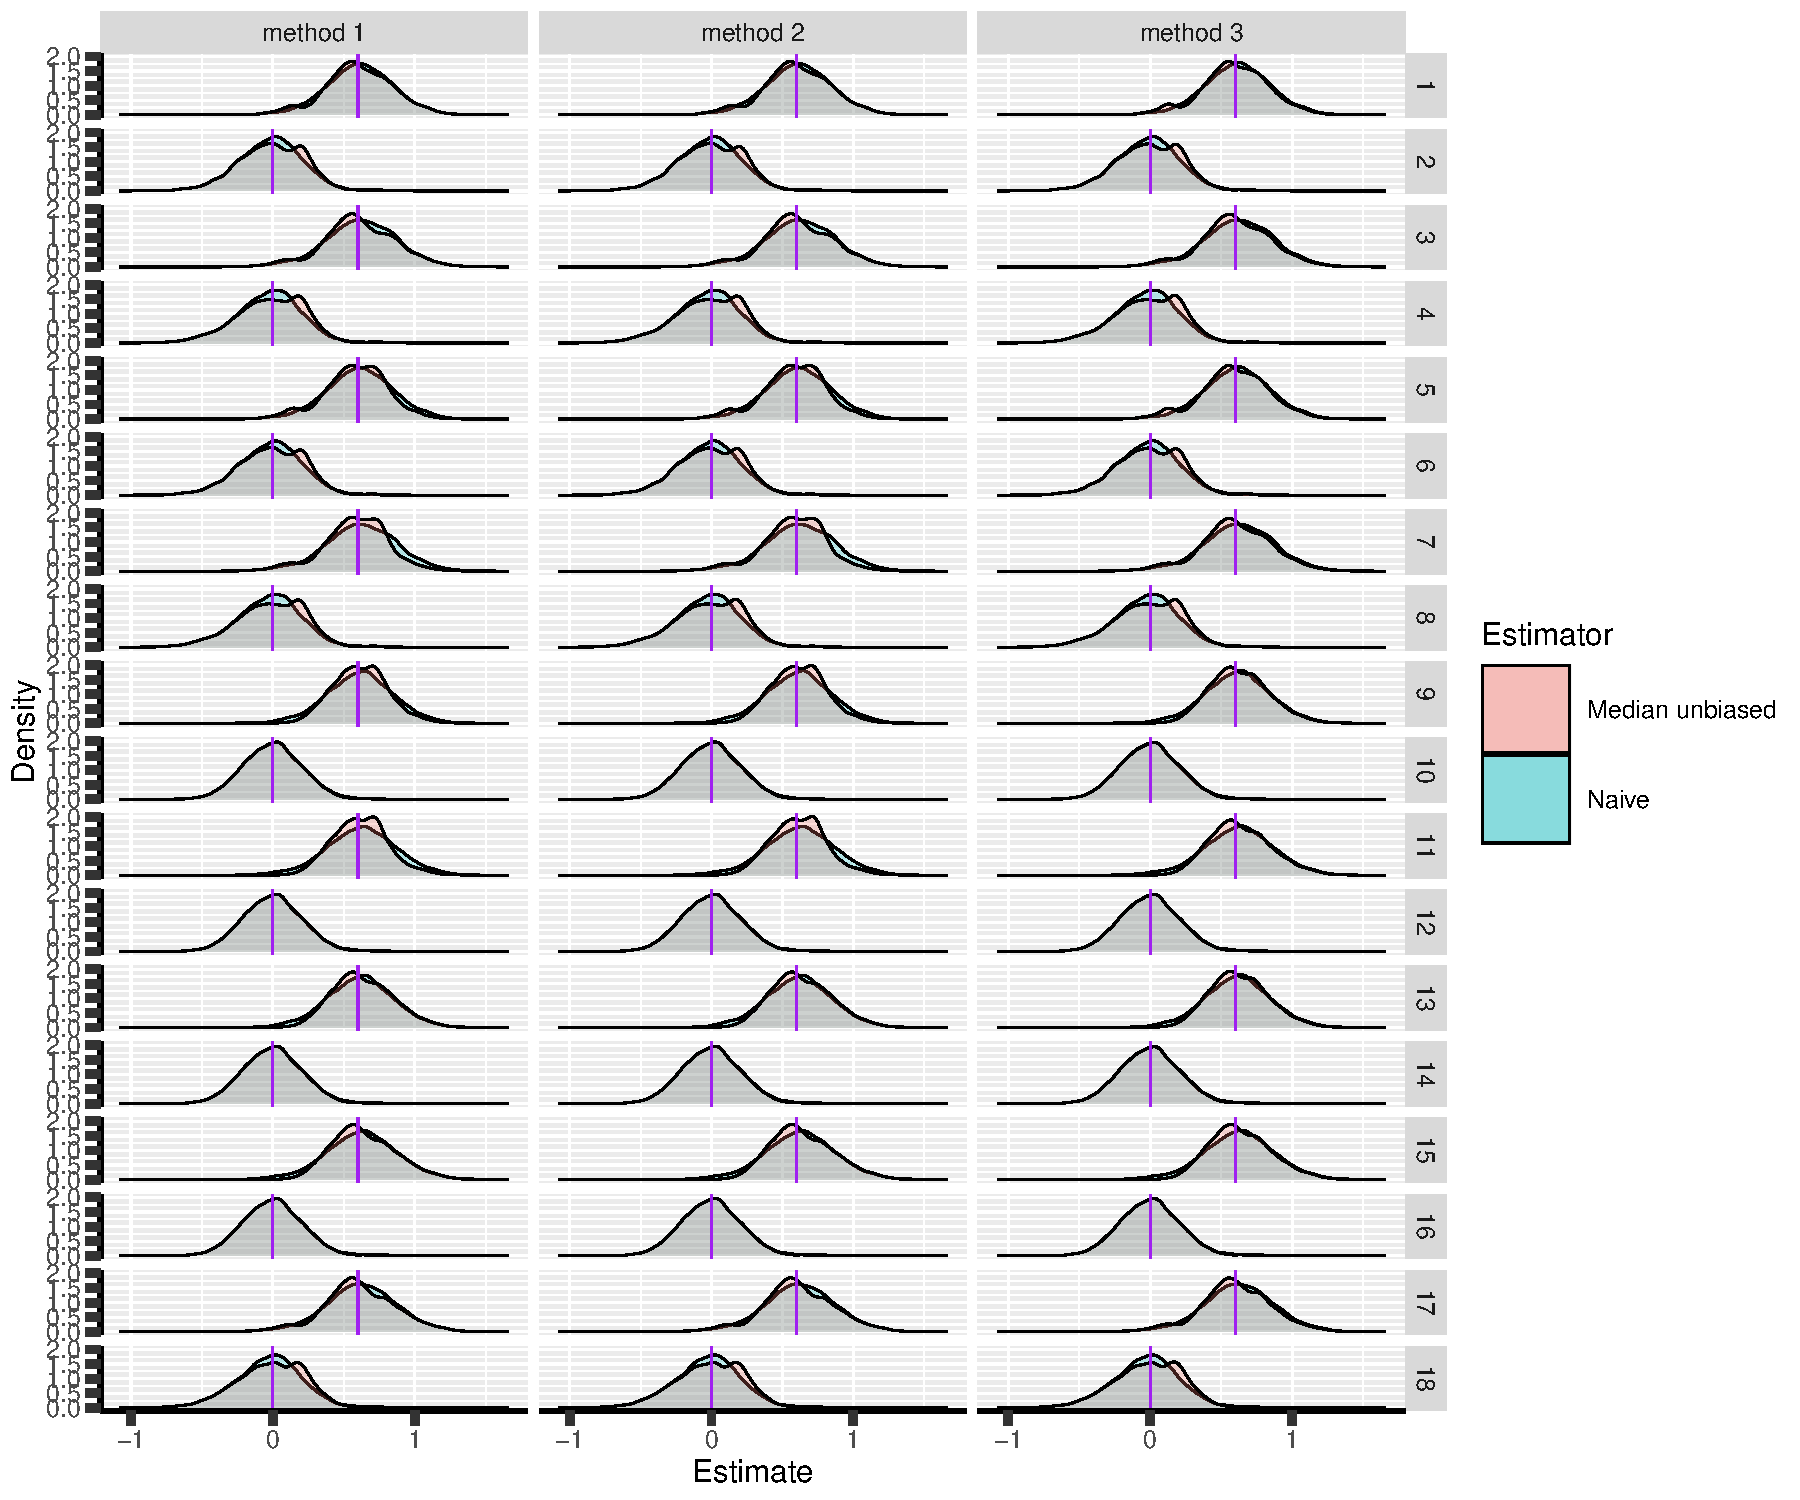
\includegraphics[trim={0 0 0 0},width=1\textwidth]{./figures/gg2stage-estimate-density.pdf}
\caption{Naive and Median unbiased estimate distribution over all simulations. Each row correspond to a different scenario}
\end{figure}

\begin{figure}[!h]
\centering
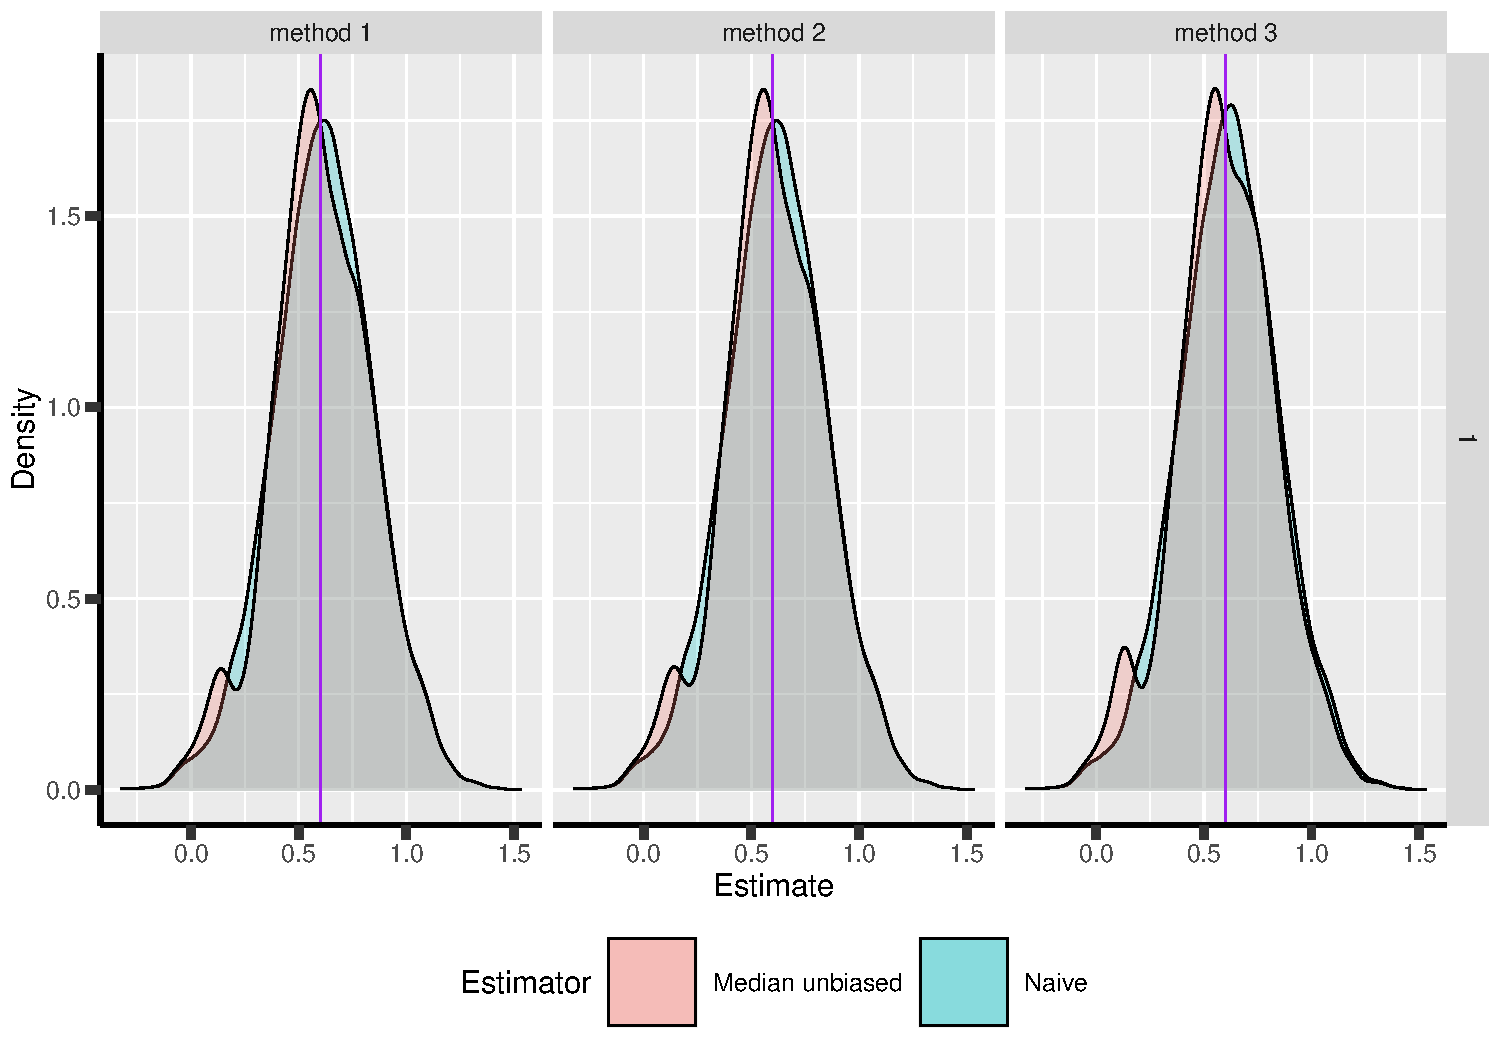
\includegraphics[trim={0 0 0 0},width=\textwidth]{./figures/gg2stage-estimate-density-scenario1.pdf}
\caption{Same but specific to scenario 1}
\end{figure}

\clearpage

Distribution of the median unbiased estimate conditional to the stage:
\begin{figure}[!h]
\centering
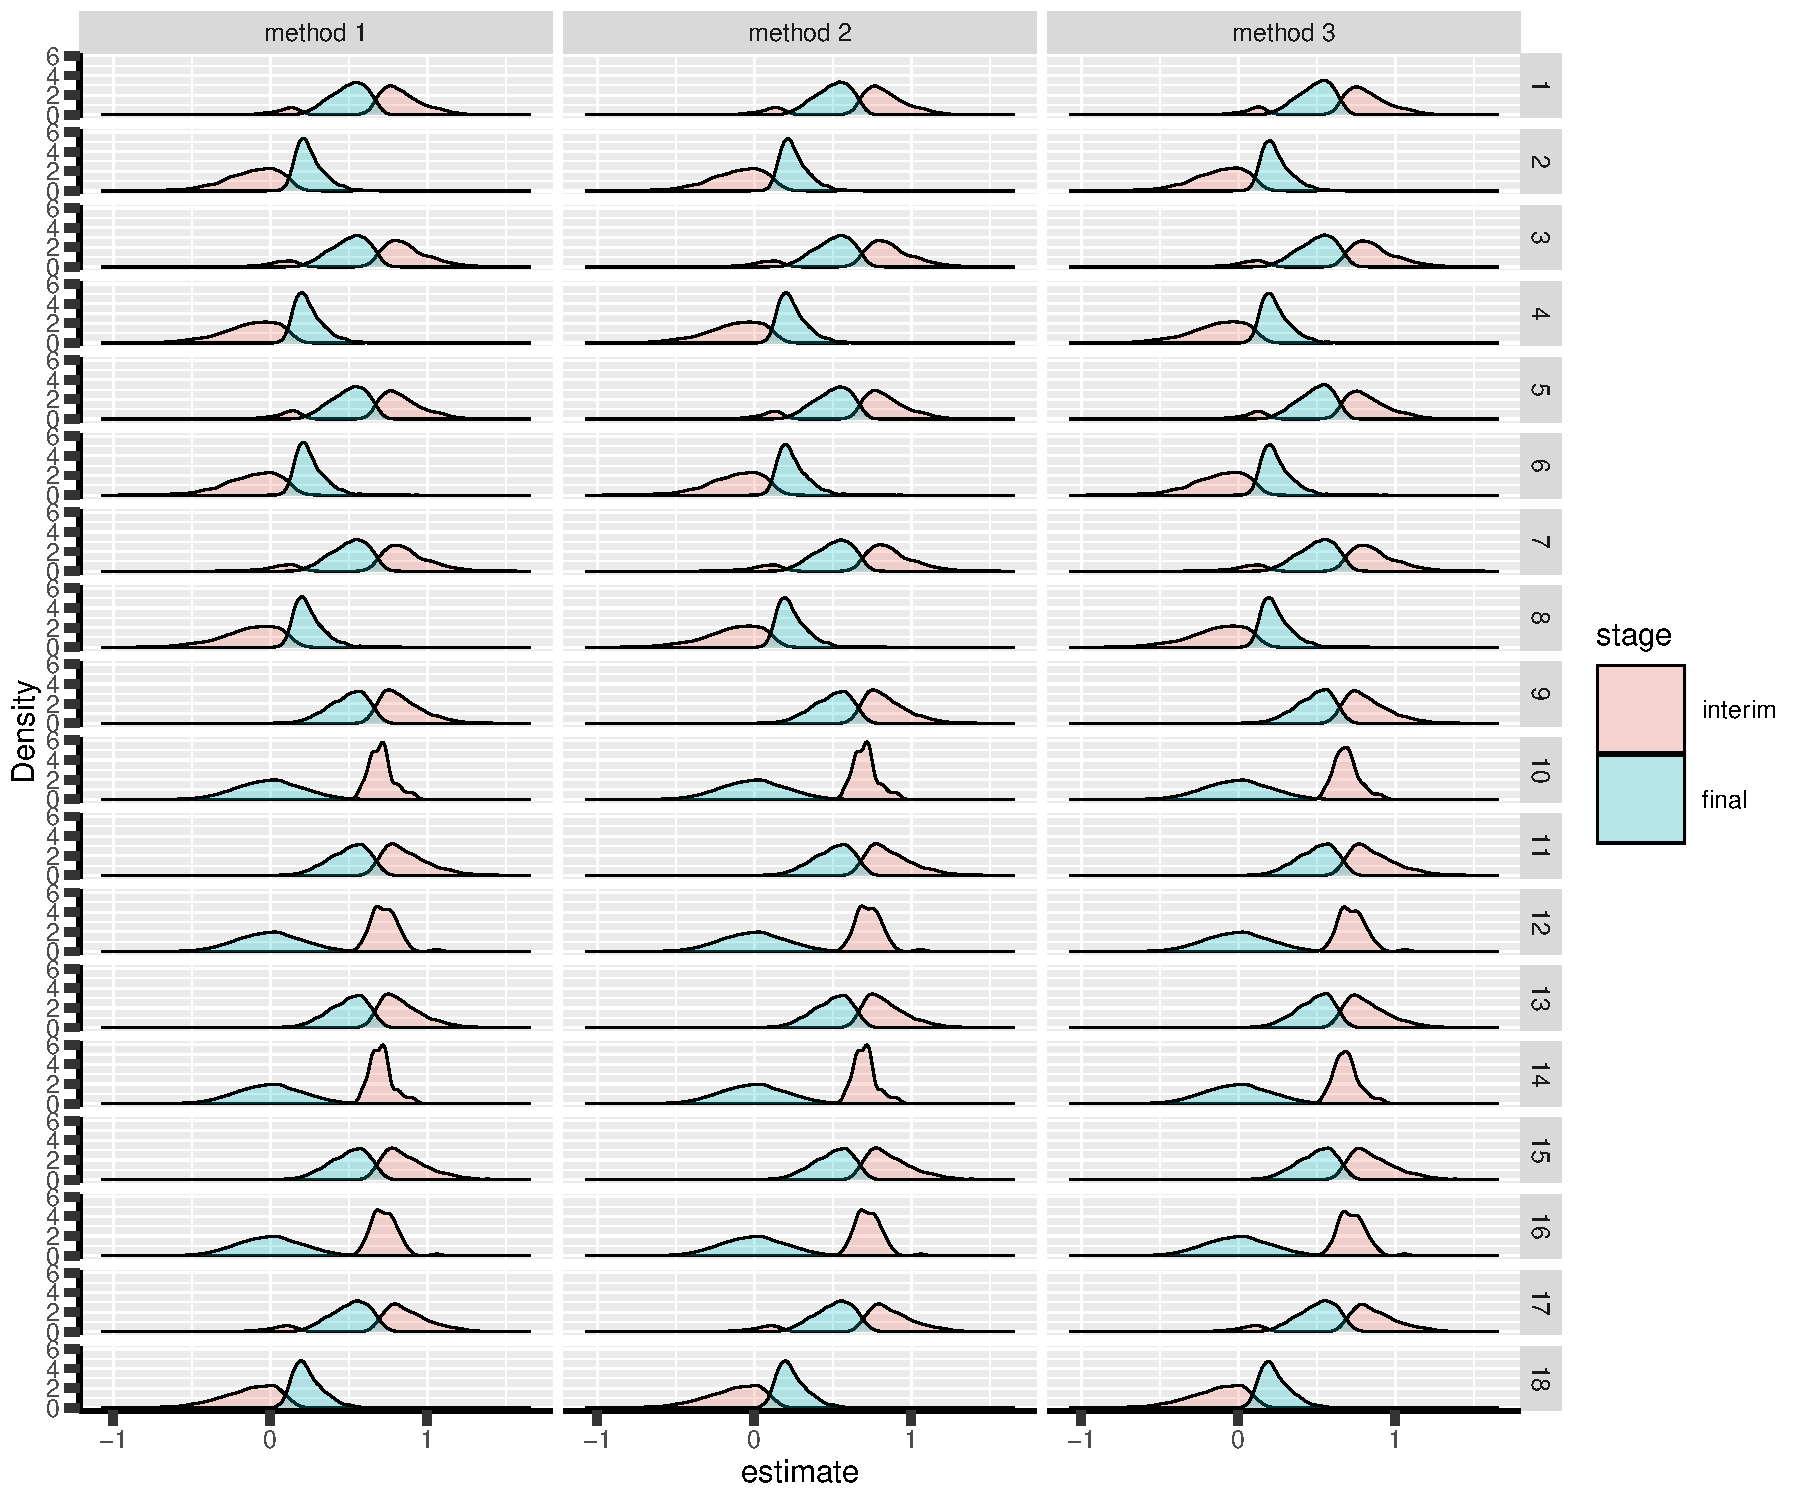
\includegraphics[trim={0 0 0 0},width=1\textwidth]{./figures/gg2stage-estimateC-density.pdf}
\caption{Median unbiased estimate distribution conditional to the stage. Each row correspond to a different scenario.}
\end{figure}

\clearpage

\subsection{3 stages}
\label{sec:org2e475a8}

Distribution of the estimates:
\begin{figure}[!h]
\centering
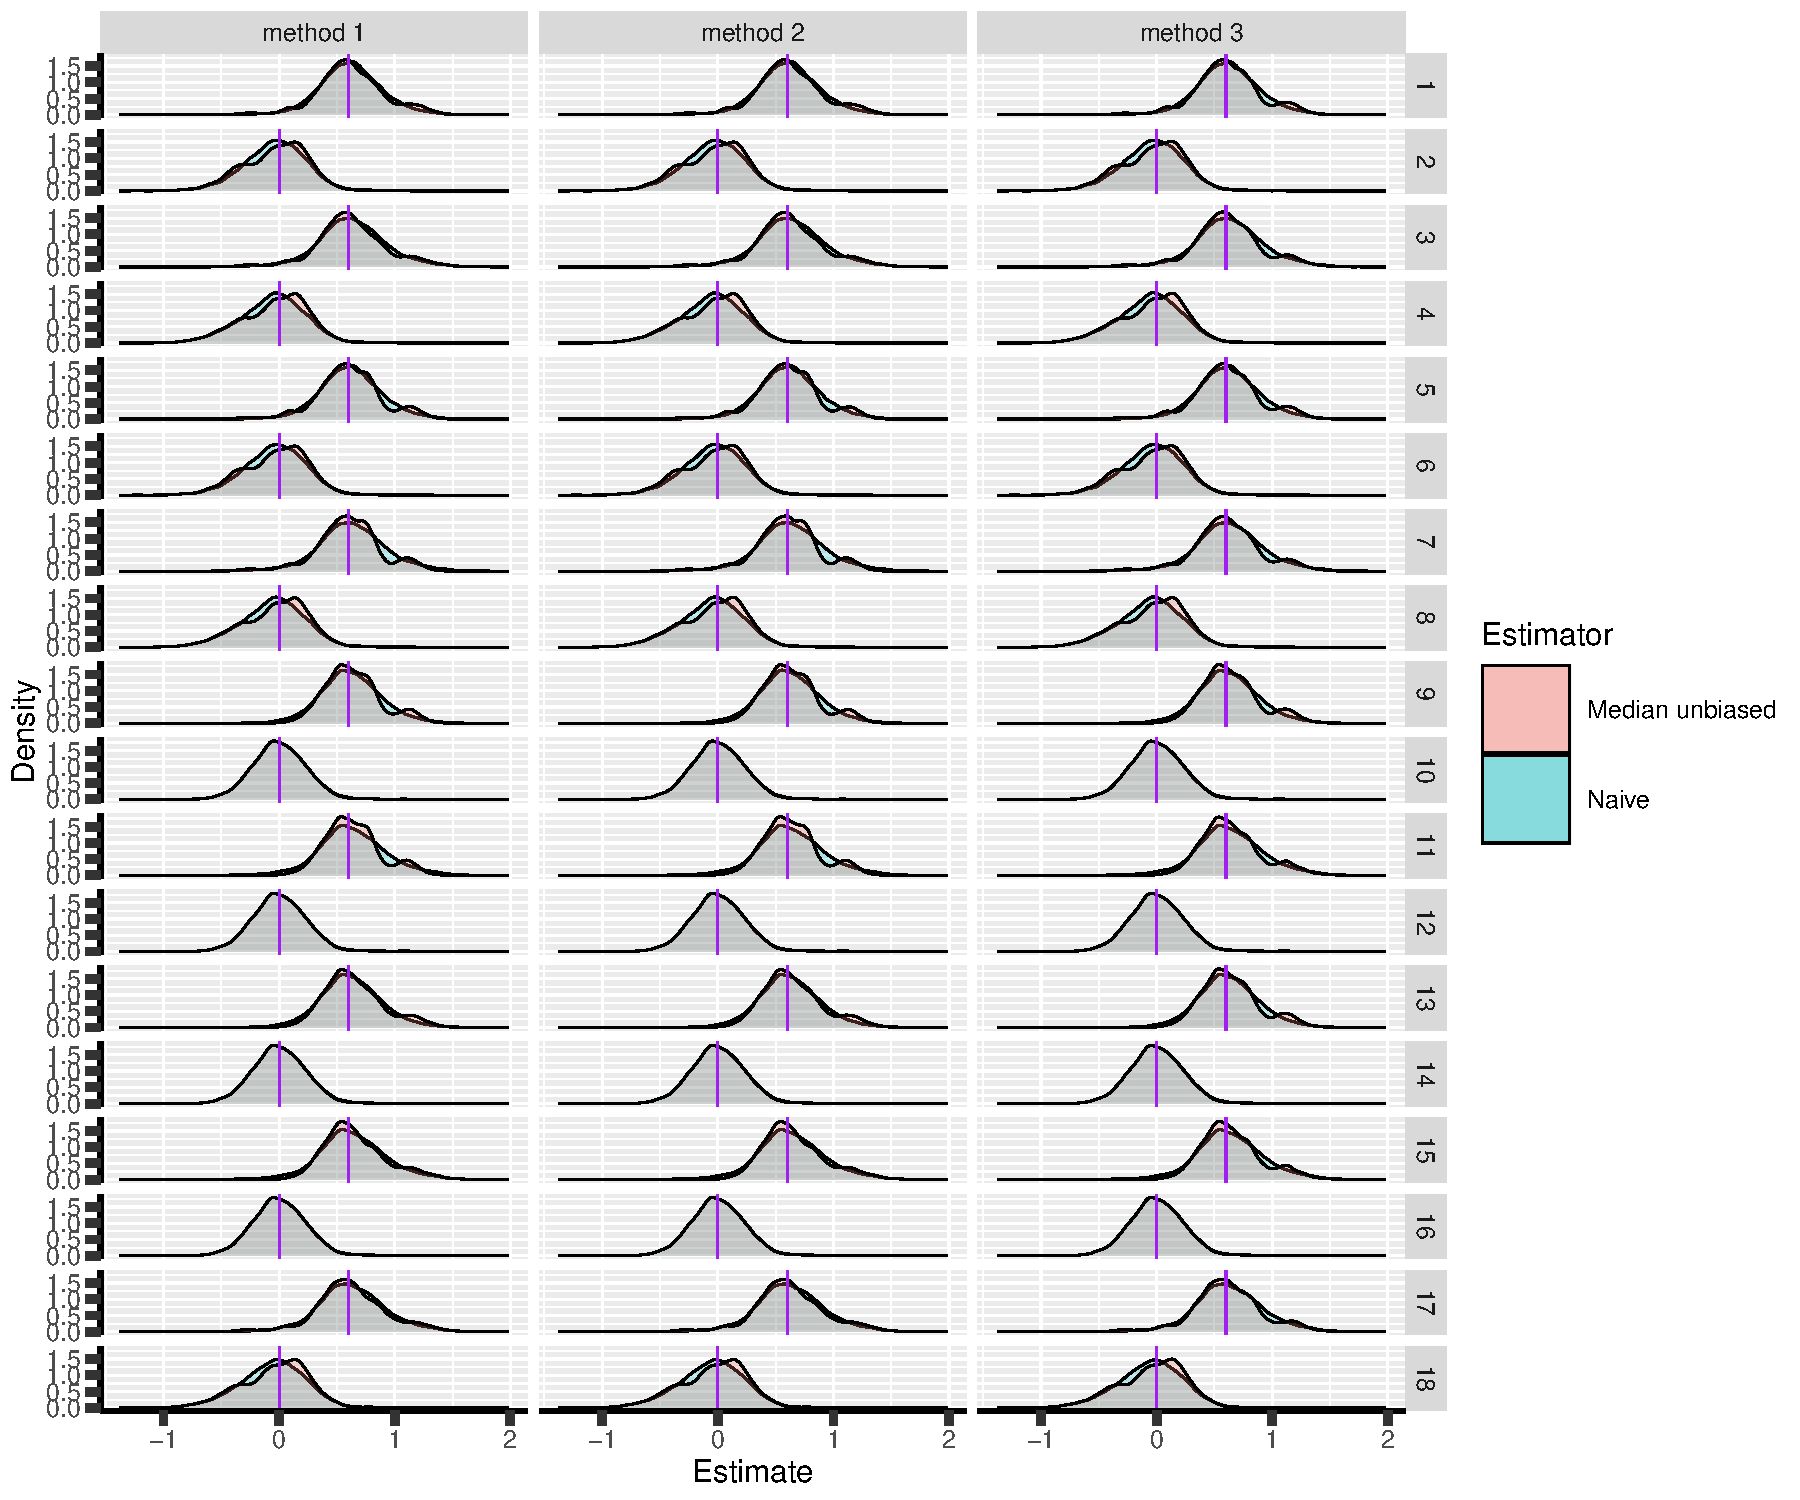
\includegraphics[trim={0 0 0 0},width=1\textwidth]{./figures/gg3stage-estimate-density.pdf}
\caption{Naive and Median unbiased estimate distribution over all simulations. Each row correspond to a different scenario}
\end{figure}

\begin{figure}[!h]
\centering
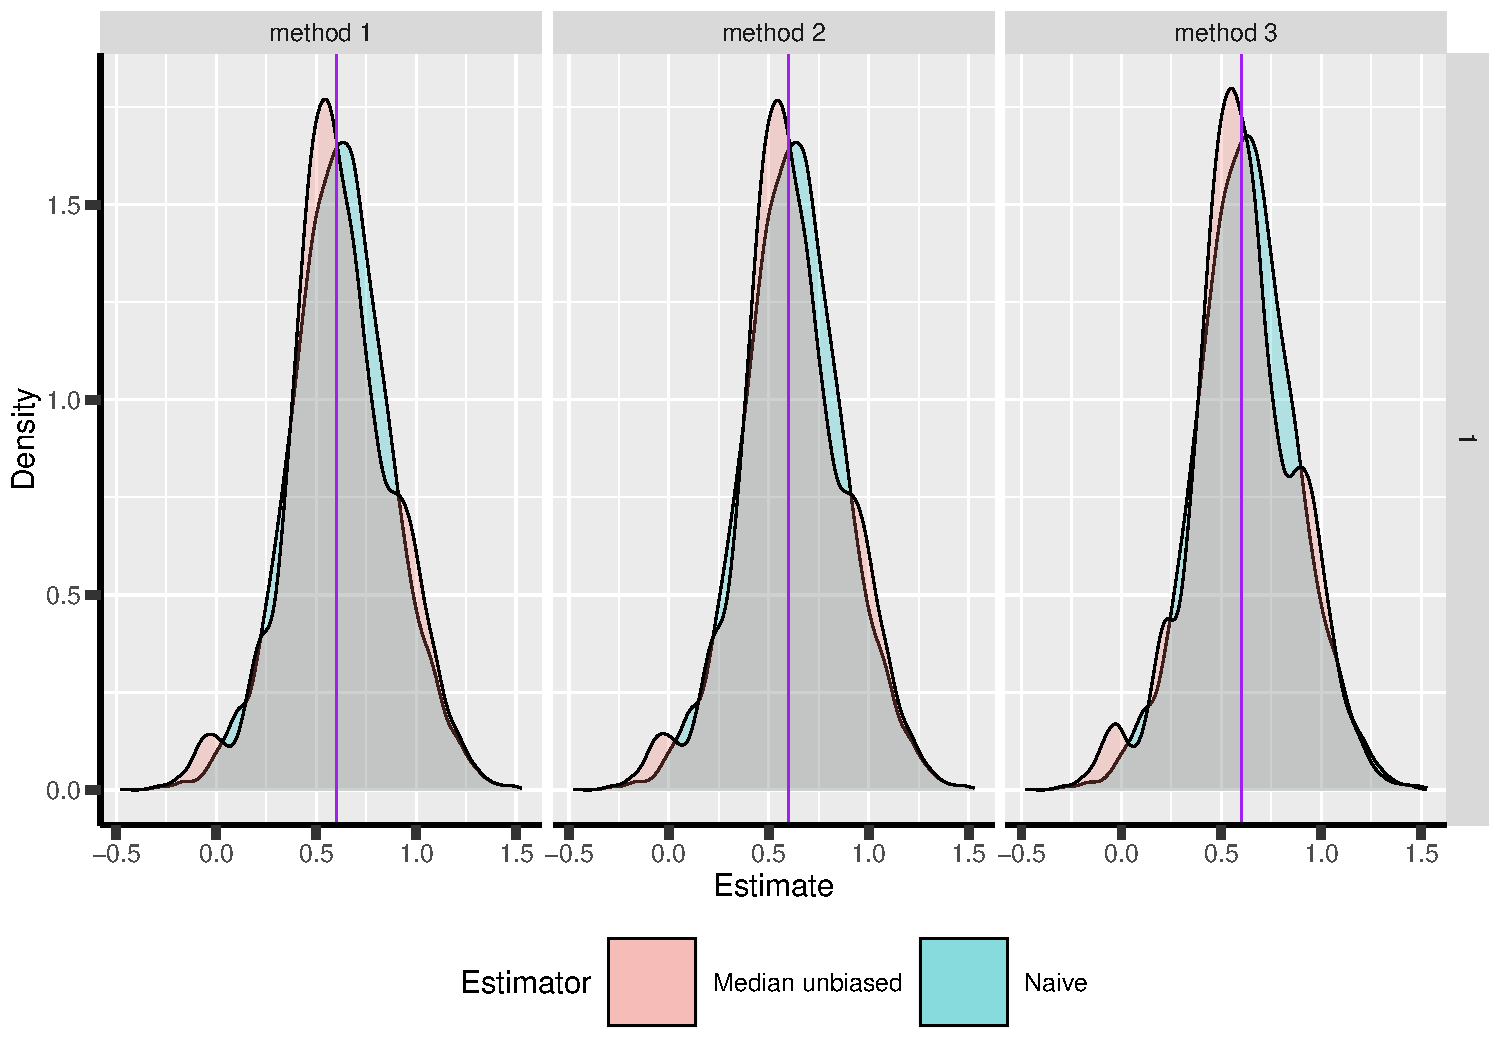
\includegraphics[trim={0 0 0 0},width=\textwidth]{./figures/gg3stage-estimate-density-scenario1.pdf}
\caption{Same but specific to scenario 1}
\end{figure}

\clearpage

Distribution of the median unbiased estimate conditional to the stage:
\begin{figure}[!h]
\centering
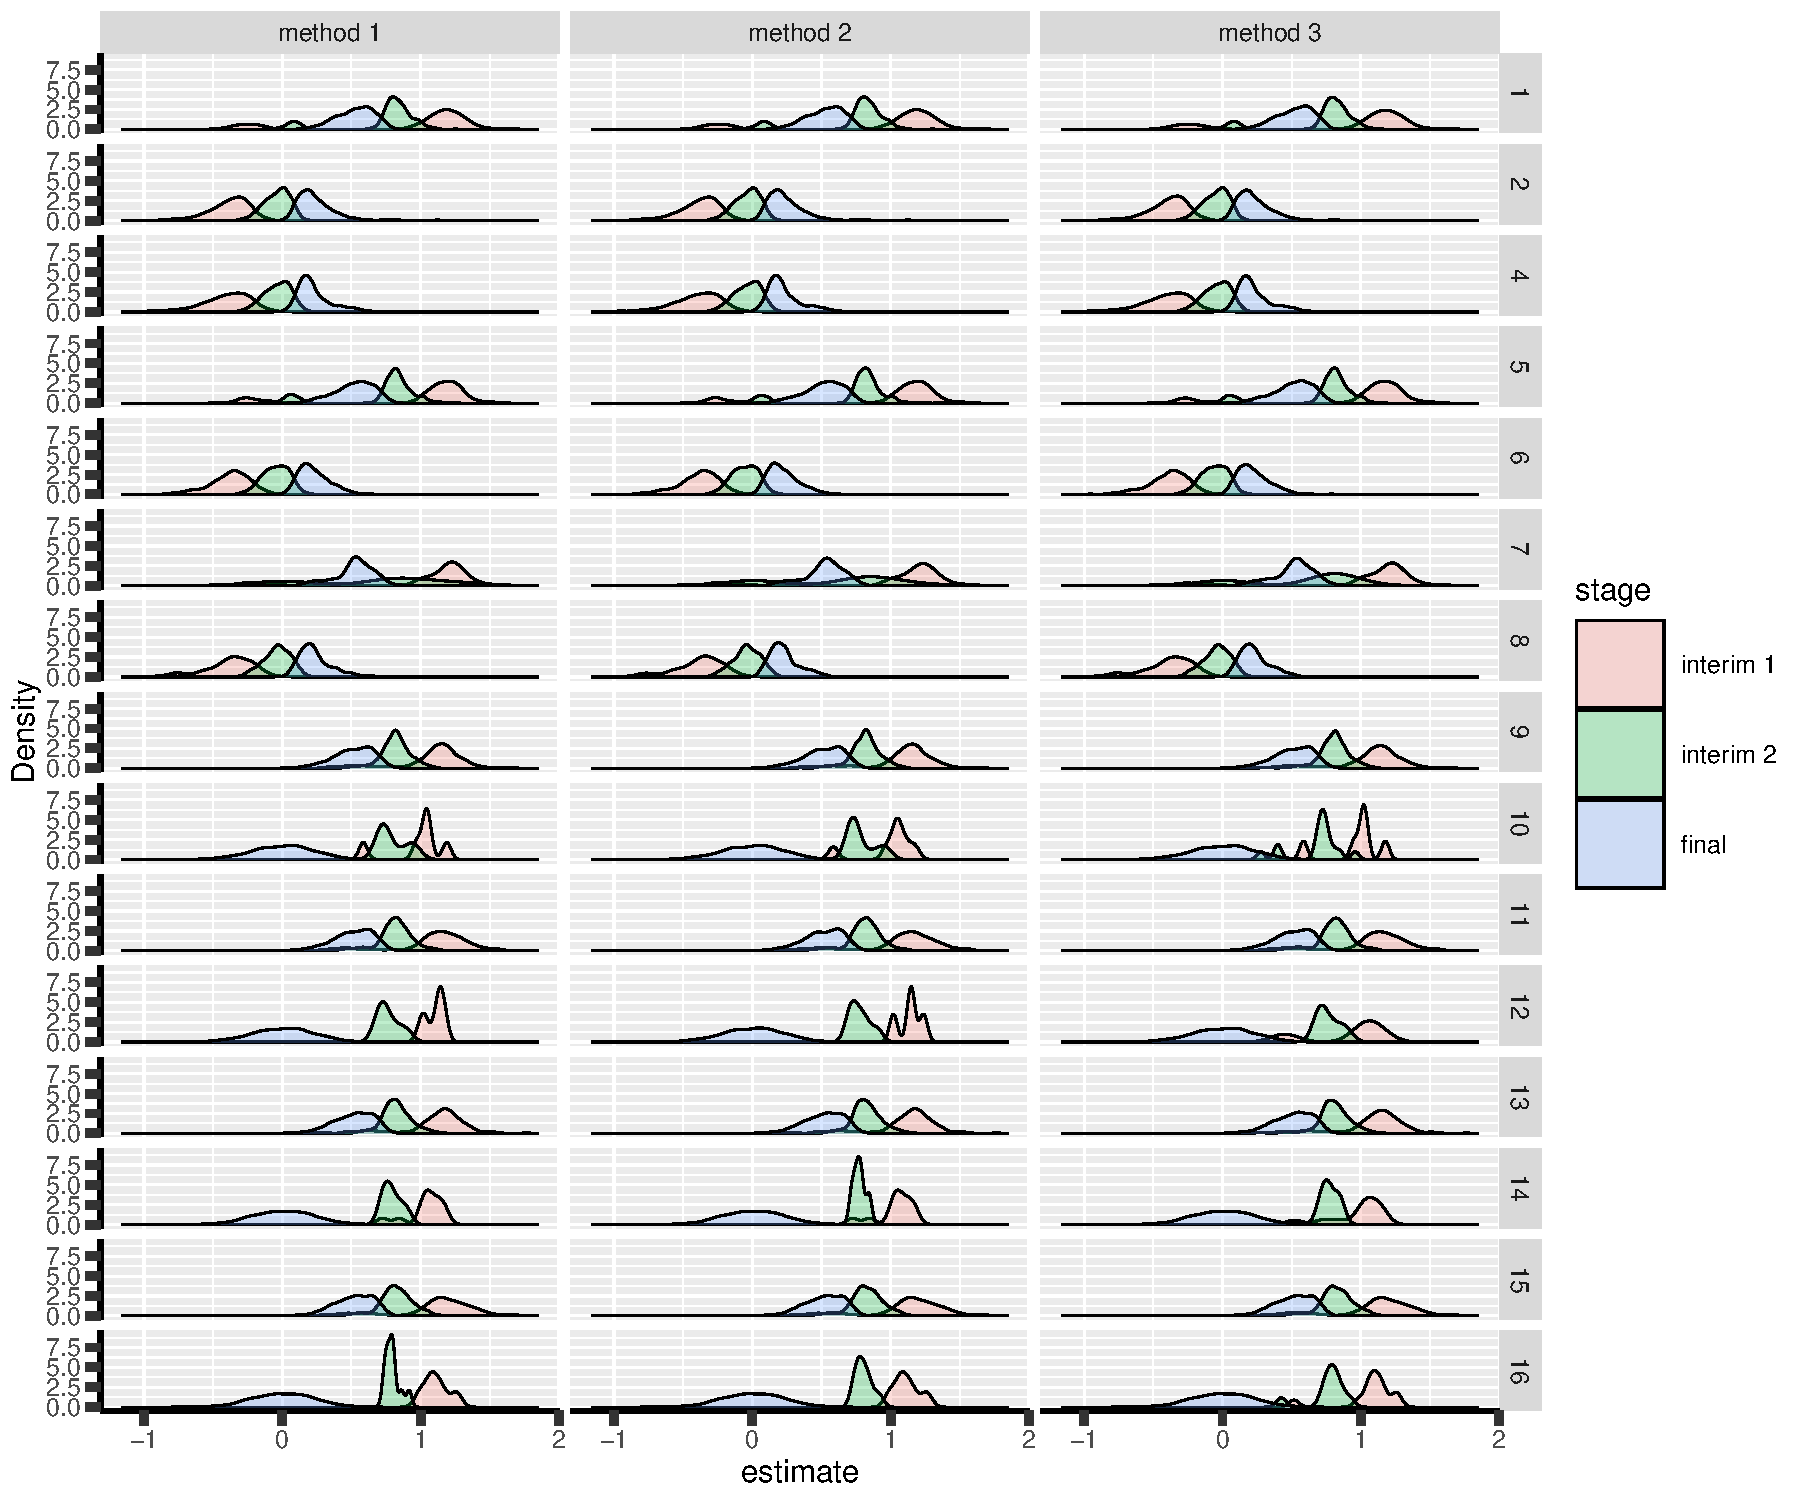
\includegraphics[trim={0 0 0 0},width=1\textwidth]{./figures/gg3stage-estimateC-density.pdf}
\caption{Median unbiased estimate distribution conditional to the stage. Each row correspond to a different scenario.}
\end{figure}

\clearpage

\section{Special cases}
\label{sec:orgd86ed90}

\subsection{2 stages}
\label{sec:org8fcd85b}

Reason for stopping (efficacy, futility, Imax reached), continuing the
trial (decreasing information, no boundary crossed), or concluding
(stop for futility at interim):
\begin{verbatim}
                                    scenario    1    2    3    4    5    6    7    8
reason                       method                                                 
decreasing information       1                  0    0    1    1    0    0    1    1
                             2                  0    0    1    1    0    0    1    1
                             3                  0    0    1    1    0    0    1    1
efficacy                     1               3739   81 3573   74 3739   81 3573   74
                             2               3744   81 3576   74 3718   79 3545   71
                             3               4165  108 3721   82 4165  108 3721   82
futility                     1                632 7111  599 6932  632 7111  599 6932
                             2                659 7161  600 6938  574 6940  562 6828
                             3                545 6844  563 6828  545 6844  563 6828
Imax reached                 1                  1    1    0    0    1    1    0    0
                             2                  1    1    0    0    1    1    0    0
                             3                  1    1    0    0    1    1    0    0
no boundary crossed          1               5628 2807 5828 2994 5628 2807 5828 2994
                             2               5596 2757 5824 2988 5707 2980 5893 3101
                             3               5289 3047 5716 3090 5289 3047 5716 3090
stop for futility at interim 1                  0    0    0    0    0    0    0    0
                             2                  0    0    0    0    0    0    0    0
                             3                 11    1    2    0   11    1    2    0
\end{verbatim}

\begin{verbatim}
                                    scenario    9   10   11   12   13   14   15   16   17   18
reason                       method                                                           
efficacy                     1               3849   81 3680   76 3849   81 3680   76 3396   74
                             2               3829   80 3661   75 3850   81 3683   76 3400   74
                             3               4238  110 3831   82 4238  110 3831   82 3528   80
futility                     1                613 7122  570 6945  613 7122  570 6945  535 6748
                             2                560 6975  541 6838  629 7164  574 6950  539 6755
                             3                516 6890  543 6842  516 6890  543 6842  496 6642
no boundary crossed          1               5538 2797 5750 2979 5538 2797 5750 2979 6069 3178
                             2               5611 2945 5798 3087 5521 2755 5743 2974 6061 3171
                             3               5246 3000 5626 3076 5246 3000 5626 3076 5976 3278
stop for futility at interim 1                  0    0    0    0    0    0    0    0    0    0
                             2                  0    0    0    0    0    0    0    0    0    0
                             3                  8    0    0    0    8    0    0    0    1    0
\end{verbatim}

\clearpage

\subsection{3 stages}
\label{sec:org34eaad7}

Reason for stopping (efficacy, futility, Imax reached), continuing the
trial (decreasing information, no boundary crossed), or concluding
(stop for futility at interim):
\begin{verbatim}
                                    scenario     1     2     3     4     5     6     7     8
reason                       method                                                         
decreasing information       1                   0     0     0     1     0     0     0     1
                             2                   0     0     0     1     0     0     0     1
                             3                   0     0     0     1     0     0     0     1
efficacy                     1                4871   107  4668   100  4871   107  4668   100
                             2                4873   107  4674   100  4846   105  4636    98
                             3                5264   136  4787   105  5264   136  4787   105
futility                     1                 854  8147   818  8048   854  8147   818  8048
                             2                 890  8198   824  8050   805  8034   772  7967
                             3                 761  7951   774  7973   761  7951   774  7973
Imax reached                 1                  28    13     0     0    28    13     0     0
                             2                  31    13     0     0    23    10     0     0
                             3                  25    15     0     0    25    15     0     0
no boundary crossed          1               11961  7071 12260  7413 11961  7071 12260  7413
                             2               11913  6996 12244  7406 12093  7359 12361  7592
                             3               11475  7452 12133  7560 11475  7452 12133  7560
stop for futility at interim 1                   0     0     0     0     0     0     0     0
                             2                   0     0     0     0     0     0     0     0
                             3                  28     2     1     0    28     2     1     0
\end{verbatim}

\begin{verbatim}
                                    scenario     9    10    11    12    13    14    15    16    17    18
reason                       method                                                                     
decreasing information       1                   0     0     1     0     0     0     1     0     0     0
                             2                   0     0     1     0     0     0     1     0     0     0
                             3                   0     0     1     0     0     0     1     0     0     0
efficacy                     1                4912   112  4794    97  4912   112  4794    97  4643   116
                             2                4890   109  4771    94  4914   112  4797    97  4648   116
                             3                5311   149  4921   110  5311   149  4921   110  4780   126
futility                     1                 841 12703   819 12404   841 12703   819 12404   814  7880
                             2                 785 12441   766 12253   860 12774   821 12416   820  7890
                             3                 741 12311   772 12273   741 12311   772 12273   768  7790
Imax reached                 1                  24    43     0     0    24    43     0     0     0     0
                             2                  18    29     0     0    25    44     0     0     0     0
                             3                  24    44     0     0    24    44     0     0     0     0
no boundary crossed          1               11791  7101 12153  7464 11791  7101 12153  7464 12487  7717
                             2               11914  7382 12250  7618 11762  7029 12147  7452 12470  7700
                             3               11314  7449 12025  7579 11314  7449 12025  7579 12332  7878
stop for futility at interim 1                   0     0     0     0     0     0     0     0     0     0
                             2                   0     0     0     0     0     0     0     0     0     0
                             3                  26     0     1     0    26     0     1     0     3     0
\end{verbatim}

\clearpage

\section{Reversal probability}
\label{sec:org45c6a85}

\subsection{2 stages}
\label{sec:org3318b02}


Percentage of time we observe a reversal:
\begin{verbatim}
        N  hypo missing ar binding  fixC fu2eff_1 fu2eff_2 fu2eff_3 eff2fu_1 eff2fu_2 eff2fu_3
 1: 10000 power    TRUE 10    TRUE FALSE    0.57%    0.61%        0    0.17%    0.20%    1.07%
 2: 10000 typeI    TRUE 10    TRUE FALSE    0.10%    0.09%        0    0.11%    0.11%    0.34%
 3: 10000 power    TRUE  5    TRUE FALSE    0.08%    0.08%        0    0.07%    0.07%    0.67%
 4: 10000 typeI    TRUE  5    TRUE FALSE    0.02%    0.02%        0    0.02%    0.02%    0.13%
 5: 10000 power    TRUE 10    TRUE  TRUE    0.22%    0.16%        0    0.67%    0.65%    1.07%
 6: 10000 typeI    TRUE 10    TRUE  TRUE    0.02%    0.01%        0    0.21%    0.21%    0.34%
 7: 10000 power    TRUE  5    TRUE  TRUE    0.02%    0.02%        0    0.46%    0.45%    0.67%
 8: 10000 typeI    TRUE  5    TRUE  TRUE        0        0        0    0.08%    0.08%    0.13%
 9: 10000 power    TRUE 10   FALSE  TRUE    0.14%    0.11%        0    0.58%    0.55%    1.04%
10: 10000 typeI    TRUE 10   FALSE  TRUE        0        0        0    0.20%    0.19%    0.33%
11: 10000 power    TRUE  5   FALSE  TRUE    0.01%    0.01%        0    0.46%    0.44%    0.60%
12: 10000 typeI    TRUE  5   FALSE  TRUE        0        0        0    0.06%    0.06%    0.09%
13: 10000 power    TRUE 10   FALSE FALSE    0.41%    0.42%        0    0.21%    0.22%    1.04%
14: 10000 typeI    TRUE 10   FALSE FALSE        0        0        0    0.12%    0.12%    0.33%
15: 10000 power    TRUE  5   FALSE FALSE    0.03%    0.03%        0    0.04%    0.04%    0.60%
16: 10000 typeI    TRUE  5   FALSE FALSE        0        0        0    0.01%    0.01%    0.09%
17: 10000 power   FALSE  5    TRUE FALSE    0.06%    0.07%        0    0.04%    0.04%    0.63%
18: 10000 typeI   FALSE  5    TRUE FALSE    0.01%    0.01%        0    0.01%    0.01%    0.12%
\end{verbatim}

\clearpage

\subsection{3 stages}
\label{sec:org4a17e99}

Percentage of time we observe a reversal:
\begin{verbatim}
        N  hypo missing ar binding  fixC fu2eff_1 fu2eff_2 fu2eff_3 eff2fu_1 eff2fu_2 eff2fu_3
 1: 10000 power    TRUE 10    TRUE FALSE    0.68%    0.69%        0    0.39%    0.41%    1.55%
 2: 10000 typeI    TRUE 10    TRUE FALSE    0.12%    0.11%        0    0.14%    0.14%    0.44%
 3:  9921 power    TRUE  5    TRUE FALSE    0.13%    0.14%        0    0.10%    0.10%    0.78%
 4: 10000 typeI    TRUE  5    TRUE FALSE        0        0        0    0.05%    0.05%    0.12%
 5: 10000 power    TRUE 10    TRUE  TRUE    0.36%    0.32%        0    1.10%    1.06%    1.55%
 6: 10000 typeI    TRUE 10    TRUE  TRUE    0.04%    0.03%        0    0.25%    0.23%    0.44%
 7:  9921 power    TRUE  5    TRUE  TRUE    0.01%    0.01%        0    0.56%    0.56%    0.78%
 8: 10000 typeI    TRUE  5    TRUE  TRUE        0        0        0    0.10%    0.10%    0.12%
 9: 10000 power    TRUE 10   FALSE  TRUE    0.36%    0.32%        0    1.00%    0.94%    1.60%
10: 10000 typeI    TRUE 10   FALSE  TRUE        0        0        0    0.30%    0.30%    0.51%
11: 10000 power    TRUE  5   FALSE  TRUE    0.02%    0.02%        0    0.54%    0.53%    0.89%
12: 10000 typeI    TRUE  5   FALSE  TRUE        0        0        0    0.14%    0.13%    0.19%
13: 10000 power    TRUE 10   FALSE FALSE    0.68%    0.69%        0    0.38%    0.39%    1.60%
14: 10000 typeI    TRUE 10   FALSE FALSE        0        0        0    0.20%    0.20%    0.51%
15: 10000 power    TRUE  5   FALSE FALSE    0.11%    0.10%        0    0.11%    0.12%    0.89%
16: 10000 typeI    TRUE  5   FALSE FALSE        0        0        0    0.01%    0.01%    0.19%
17: 10000 power   FALSE  5    TRUE FALSE    0.15%    0.14%        0    0.05%    0.05%    0.70%
18: 10000 typeI   FALSE  5    TRUE FALSE    0.06%    0.06%        0    0.03%    0.03%    0.17%
\end{verbatim}


\clearpage

\section{Logical consistency of p-values/CIs}
\label{sec:org212961d}

\subsection{Mismatch p-value / boundaries}
\label{sec:org9d927a6}
\subsubsection{2 stages}
\label{sec:orgb3eaca8}

When concluding for futility:
\begin{verbatim}
     hypo missing ar binding  fixC method 1 method 2 method 3
 1: power    TRUE 10    TRUE FALSE        0        0        0
 2: typeI    TRUE 10    TRUE FALSE        0        0        0
 3: power    TRUE  5    TRUE FALSE        0        0        0
 4: typeI    TRUE  5    TRUE FALSE        0        0        0
 5: power    TRUE 10    TRUE  TRUE        0        0        0
 6: typeI    TRUE 10    TRUE  TRUE        0        0        0
 7: power    TRUE  5    TRUE  TRUE        0        0        0
 8: typeI    TRUE  5    TRUE  TRUE        0        0        0
 9: power    TRUE 10   FALSE  TRUE        0        0        0
10: typeI    TRUE 10   FALSE  TRUE        0        0        0
11: power    TRUE  5   FALSE  TRUE        0        0        0
12: typeI    TRUE  5   FALSE  TRUE        0        0        0
13: power    TRUE 10   FALSE FALSE        0        0        0
14: typeI    TRUE 10   FALSE FALSE        0        0        0
15: power    TRUE  5   FALSE FALSE        0        0        0
16: typeI    TRUE  5   FALSE FALSE        0        0        0
17: power   FALSE  5    TRUE FALSE        0        0        0
18: typeI   FALSE  5    TRUE FALSE        0        0        0
\end{verbatim}

When concluding for efficacy:
\begin{verbatim}
     hypo missing ar binding  fixC method 1 method 2 method 3
 1: power    TRUE 10    TRUE FALSE        0        0        0
 2: typeI    TRUE 10    TRUE FALSE        0        0        0
 3: power    TRUE  5    TRUE FALSE        0        0        0
 4: typeI    TRUE  5    TRUE FALSE        0        0        0
 5: power    TRUE 10    TRUE  TRUE        0        0        0
 6: typeI    TRUE 10    TRUE  TRUE        0        0        0
 7: power    TRUE  5    TRUE  TRUE        0        0        0
 8: typeI    TRUE  5    TRUE  TRUE        0        0        0
 9: power    TRUE 10   FALSE  TRUE        0        0        0
10: typeI    TRUE 10   FALSE  TRUE        0        0        0
11: power    TRUE  5   FALSE  TRUE        0        0        0
12: typeI    TRUE  5   FALSE  TRUE        0        0        0
13: power    TRUE 10   FALSE FALSE        0        0        0
14: typeI    TRUE 10   FALSE FALSE        0        0        0
15: power    TRUE  5   FALSE FALSE        0        0        0
16: typeI    TRUE  5   FALSE FALSE        0        0        0
17: power   FALSE  5    TRUE FALSE        0        0        0
18: typeI   FALSE  5    TRUE FALSE        0        0        0
\end{verbatim}

\clearpage

\subsubsection{3 stages}
\label{sec:org77f7b50}

When concluding for futility:
\begin{verbatim}
     hypo missing ar binding  fixC method 1 method 2 method 3
 1: power    TRUE 10    TRUE FALSE        0    0.05%        0
 2: typeI    TRUE 10    TRUE FALSE        0        0        0
 3: power    TRUE  5    TRUE FALSE        0        0        0
 4: typeI    TRUE  5    TRUE FALSE        0        0        0
 5: power    TRUE 10    TRUE  TRUE        0        0        0
 6: typeI    TRUE 10    TRUE  TRUE        0        0        0
 7: power    TRUE  5    TRUE  TRUE        0        0        0
 8: typeI    TRUE  5    TRUE  TRUE        0        0        0
 9: power    TRUE 10   FALSE  TRUE        0    0.05%        0
10: typeI    TRUE 10   FALSE  TRUE        0        0        0
11: power    TRUE  5   FALSE  TRUE        0        0        0
12: typeI    TRUE  5   FALSE  TRUE        0        0    0.01%
13: power    TRUE 10   FALSE FALSE        0        0        0
14: typeI    TRUE 10   FALSE FALSE        0        0        0
15: power    TRUE  5   FALSE FALSE        0        0    0.05%
16: typeI    TRUE  5   FALSE FALSE        0        0    0.01%
17: power   FALSE  5    TRUE FALSE        0        0        0
18: typeI   FALSE  5    TRUE FALSE        0        0        0
\end{verbatim}

Largest mismatch:
\begin{verbatim}
[1] 0.02499569043
\end{verbatim}



When concluding for efficacy:
\begin{verbatim}
     hypo missing ar binding  fixC method 1 method 2 method 3
 1: power    TRUE 10    TRUE FALSE        0        0        0
 2: typeI    TRUE 10    TRUE FALSE        0        0        0
 3: power    TRUE  5    TRUE FALSE        0        0        0
 4: typeI    TRUE  5    TRUE FALSE        0        0        0
 5: power    TRUE 10    TRUE  TRUE        0        0        0
 6: typeI    TRUE 10    TRUE  TRUE        0        0        0
 7: power    TRUE  5    TRUE  TRUE        0        0    0.01%
 8: typeI    TRUE  5    TRUE  TRUE        0        0        0
 9: power    TRUE 10   FALSE  TRUE        0        0        0
10: typeI    TRUE 10   FALSE  TRUE        0        0        0
11: power    TRUE  5   FALSE  TRUE        0        0        0
12: typeI    TRUE  5   FALSE  TRUE        0        0        0
13: power    TRUE 10   FALSE FALSE        0    0.01%    0.01%
14: typeI    TRUE 10   FALSE FALSE        0        0        0
15: power    TRUE  5   FALSE FALSE        0        0        0
16: typeI    TRUE  5   FALSE FALSE        0        0        0
17: power   FALSE  5    TRUE FALSE        0        0        0
18: typeI   FALSE  5    TRUE FALSE        0        0    0.40%
\end{verbatim}

Largest mismatch:
\begin{verbatim}
[1] 0.02500297183
\end{verbatim}


\clearpage

\subsection{Mismatch confidence intervals / boundaries}
\label{sec:orgd20c866}

\subsubsection{2 stages}
\label{sec:org3918c47}

When concluding for futility:
\begin{verbatim}
     hypo missing ar binding  fixC       method 1       method 2       method 3
 1: power    TRUE 10    TRUE FALSE              0              0  0 (NA: 0.05%)
 2: typeI    TRUE 10    TRUE FALSE              0              0              0
 3: power    TRUE  5    TRUE FALSE              0              0              0
 4: typeI    TRUE  5    TRUE FALSE              0              0              0
 5: power    TRUE 10    TRUE  TRUE              0              0  0 (NA: 0.05%)
 6: typeI    TRUE 10    TRUE  TRUE              0              0              0
 7: power    TRUE  5    TRUE  TRUE              0              0              0
 8: typeI    TRUE  5    TRUE  TRUE              0              0              0
 9: power    TRUE 10   FALSE  TRUE 0 (NA: 32.62%) 0 (NA: 30.38%) 0 (NA: 31.41%)
10: typeI    TRUE 10   FALSE  TRUE  0 (NA: 0.21%)  0 (NA: 0.19%)  0 (NA: 0.34%)
11: power    TRUE  5   FALSE  TRUE 0 (NA: 30.64%) 0 (NA: 29.26%) 0 (NA: 30.24%)
12: typeI    TRUE  5   FALSE  TRUE  0 (NA: 0.06%)  0 (NA: 0.06%)  0 (NA: 0.09%)
13: power    TRUE 10   FALSE FALSE 0 (NA: 30.41%) 0 (NA: 31.13%) 0 (NA: 31.41%)
14: typeI    TRUE 10   FALSE FALSE  0 (NA: 0.12%)  0 (NA: 0.12%)  0 (NA: 0.34%)
15: power    TRUE  5   FALSE FALSE 0 (NA: 29.09%) 0 (NA: 29.28%) 0 (NA: 30.24%)
16: typeI    TRUE  5   FALSE FALSE  0 (NA: 0.01%)  0 (NA: 0.01%)  0 (NA: 0.09%)
17: power   FALSE  5    TRUE FALSE              0              0              0
18: typeI   FALSE  5    TRUE FALSE              0              0              0
\end{verbatim}

When concluding for efficacy:
\begin{verbatim}
     hypo missing ar binding  fixC      method 1      method 2      method 3
 1: power    TRUE 10    TRUE FALSE 0 (NA: 0.02%) 0 (NA: 0.02%) 0 (NA: 0.01%)
 2: typeI    TRUE 10    TRUE FALSE             0             0             0
 3: power    TRUE  5    TRUE FALSE             0             0             0
 4: typeI    TRUE  5    TRUE FALSE             0             0             0
 5: power    TRUE 10    TRUE  TRUE 0 (NA: 0.02%) 0 (NA: 0.02%) 0 (NA: 0.01%)
 6: typeI    TRUE 10    TRUE  TRUE             0             0             0
 7: power    TRUE  5    TRUE  TRUE             0             0             0
 8: typeI    TRUE  5    TRUE  TRUE             0             0             0
 9: power    TRUE 10   FALSE  TRUE 0 (NA: 0.03%) 0 (NA: 0.02%) 0 (NA: 0.01%)
10: typeI    TRUE 10   FALSE  TRUE             0             0             0
11: power    TRUE  5   FALSE  TRUE 0 (NA: 0.01%) 0 (NA: 0.02%) 0 (NA: 0.02%)
12: typeI    TRUE  5   FALSE  TRUE             0             0             0
13: power    TRUE 10   FALSE FALSE 0 (NA: 0.02%) 0 (NA: 0.02%) 0 (NA: 0.01%)
14: typeI    TRUE 10   FALSE FALSE             0             0             0
15: power    TRUE  5   FALSE FALSE 0 (NA: 0.01%) 0 (NA: 0.01%) 0 (NA: 0.02%)
16: typeI    TRUE  5   FALSE FALSE             0             0             0
17: power   FALSE  5    TRUE FALSE 0 (NA: 0.02%) 0 (NA: 0.02%) 0 (NA: 0.03%)
18: typeI   FALSE  5    TRUE FALSE             0             0             0
\end{verbatim}

\subsubsection{3 stages}
\label{sec:org919099c}

When concluding for futility:
\begin{verbatim}
     hypo missing ar binding  fixC           method 1           method 2          method 3
 1: power    TRUE 10    TRUE FALSE                  0                  0     0 (NA: 0.60%)
 2: typeI    TRUE 10    TRUE FALSE                  0                  0     0 (NA: 0.02%)
 3: power    TRUE  5    TRUE FALSE                  0                  0 0.05% (NA: 0.10%)
 4: typeI    TRUE  5    TRUE FALSE                  0                  0                 0
 5: power    TRUE 10    TRUE  TRUE      0 (NA: 0.30%)      0 (NA: 0.45%)     0 (NA: 0.60%)
 6: typeI    TRUE 10    TRUE  TRUE      0 (NA: 0.02%)      0 (NA: 0.02%)     0 (NA: 0.02%)
 7: power    TRUE  5    TRUE  TRUE      0 (NA: 0.05%)  0.05% (NA: 0.05%)     0 (NA: 0.10%)
 8: typeI    TRUE  5    TRUE  TRUE                  0                  0                 0
 9: power    TRUE 10   FALSE  TRUE     0 (NA: 44.32%)     0 (NA: 42.22%)    0 (NA: 45.19%)
10: typeI    TRUE 10   FALSE  TRUE      0 (NA: 0.31%)      0 (NA: 0.33%)     0 (NA: 0.52%)
11: power    TRUE  5   FALSE  TRUE 0.09% (NA: 43.38%)     0 (NA: 41.16%)    0 (NA: 42.96%)
12: typeI    TRUE  5   FALSE  TRUE      0 (NA: 0.14%)      0 (NA: 0.13%) 0.01% (NA: 0.19%)
13: power    TRUE 10   FALSE FALSE     0 (NA: 41.63%)     0 (NA: 42.43%)    0 (NA: 45.19%)
14: typeI    TRUE 10   FALSE FALSE      0 (NA: 0.21%)      0 (NA: 0.23%)     0 (NA: 0.52%)
15: power    TRUE  5   FALSE FALSE 0.09% (NA: 41.87%) 0.09% (NA: 42.03%)    0 (NA: 42.96%)
16: typeI    TRUE  5   FALSE FALSE      0 (NA: 0.01%)      0 (NA: 0.01%)     0 (NA: 0.19%)
17: power   FALSE  5    TRUE FALSE                  0                  0     0 (NA: 0.20%)
18: typeI   FALSE  5    TRUE FALSE                  0                  0                 0
\end{verbatim}


Largest mismatch:
\begin{verbatim}
[1] 0.002466353937
\end{verbatim}


When concluding for efficacy:
\begin{verbatim}
     hypo missing ar binding  fixC          method 1          method 2          method 3
 1: power    TRUE 10    TRUE FALSE     0 (NA: 0.04%)     0 (NA: 0.04%)                 0
 2: typeI    TRUE 10    TRUE FALSE                 0                 0                 0
 3: power    TRUE  5    TRUE FALSE     0 (NA: 0.01%)     0 (NA: 0.03%)     0 (NA: 0.01%)
 4: typeI    TRUE  5    TRUE FALSE                 0             0.41%                 0
 5: power    TRUE 10    TRUE  TRUE     0 (NA: 0.04%)     0 (NA: 0.02%)                 0
 6: typeI    TRUE 10    TRUE  TRUE                 0                 0                 0
 7: power    TRUE  5    TRUE  TRUE     0 (NA: 0.01%)     0 (NA: 0.03%)     0 (NA: 0.01%)
 8: typeI    TRUE  5    TRUE  TRUE                 0                 0                 0
 9: power    TRUE 10   FALSE  TRUE 0.01% (NA: 0.01%)     0 (NA: 0.01%) 0.01% (NA: 0.01%)
10: typeI    TRUE 10   FALSE  TRUE                 0                 0                 0
11: power    TRUE  5   FALSE  TRUE     0 (NA: 0.01%)     0 (NA: 0.01%)     0 (NA: 0.01%)
12: typeI    TRUE  5   FALSE  TRUE                 0                 0                 0
13: power    TRUE 10   FALSE FALSE 0.01% (NA: 0.01%) 0.01% (NA: 0.01%) 0.01% (NA: 0.01%)
14: typeI    TRUE 10   FALSE FALSE                 0                 0                 0
15: power    TRUE  5   FALSE FALSE     0 (NA: 0.01%)     0 (NA: 0.01%) 0.01% (NA: 0.01%)
16: typeI    TRUE  5   FALSE FALSE                 0                 0                 0
17: power   FALSE  5    TRUE FALSE     0 (NA: 0.01%)     0 (NA: 0.01%) 0.01% (NA: 0.01%)
18: typeI   FALSE  5    TRUE FALSE             0.39%                 0                 0
\end{verbatim}

\begin{verbatim}
[1] -0.005759153782
\end{verbatim}

\subsection{Range of p-values}
\label{sec:org59d0ca4}

\subsubsection{2 stages}
\label{sec:org0c7efe1}
\begin{verbatim}
    missing binding  fixC ar  hypo       method 1       method 2       method 3
 1:    TRUE    TRUE FALSE 10 power     [0;0.9147]     [0;0.9147]     [0;0.9147]
 2:    TRUE    TRUE FALSE 10 typeI [1e-04;0.9999] [1e-04;0.9999] [1e-04;0.9999]
 3:    TRUE    TRUE FALSE  5 power     [0;0.9015]     [0;0.9015]     [0;0.9015]
 4:    TRUE    TRUE FALSE  5 typeI [1e-04;0.9998] [1e-04;0.9998] [1e-04;0.9998]
 5:    TRUE    TRUE  TRUE 10 power     [0;0.9147]     [0;0.9147]     [0;0.9147]
 6:    TRUE    TRUE  TRUE 10 typeI [2e-04;0.9999] [2e-04;0.9999] [1e-04;0.9999]
 7:    TRUE    TRUE  TRUE  5 power     [0;0.9015]     [0;0.9015]     [0;0.9015]
 8:    TRUE    TRUE  TRUE  5 typeI [3e-04;0.9998] [3e-04;0.9998] [1e-04;0.9998]
 9:    TRUE   FALSE  TRUE 10 power          [0;1]          [0;1]          [0;1]
10:    TRUE   FALSE  TRUE 10 typeI      [1e-04;1]      [1e-04;1]      [1e-04;1]
11:    TRUE   FALSE  TRUE  5 power          [0;1]          [0;1]          [0;1]
12:    TRUE   FALSE  TRUE  5 typeI      [2e-04;1]      [2e-04;1]      [1e-04;1]
13:    TRUE   FALSE FALSE 10 power          [0;1]          [0;1]          [0;1]
14:    TRUE   FALSE FALSE 10 typeI      [1e-04;1]      [1e-04;1]      [1e-04;1]
15:    TRUE   FALSE FALSE  5 power          [0;1]          [0;1]          [0;1]
16:    TRUE   FALSE FALSE  5 typeI          [0;1]          [0;1]      [1e-04;1]
17:   FALSE    TRUE FALSE  5 power     [0;0.9642]     [0;0.9642]     [0;0.9642]
18:   FALSE    TRUE FALSE  5 typeI          [0;1]          [0;1]      [1e-04;1]
\end{verbatim}

\clearpage

\subsubsection{3 stages}
\label{sec:orge2f50c4}
\begin{verbatim}
    missing binding  fixC ar  hypo       method 1       method 2       method 3
 1:    TRUE    TRUE FALSE 10 power     [0;0.9547]     [0;0.9547]     [0;0.9547]
 2:    TRUE    TRUE FALSE 10 typeI [2e-04;0.9999] [2e-04;0.9999] [4e-04;0.9999]
 3:    TRUE    TRUE FALSE  5 power     [0;0.9954]     [0;0.9954]     [0;0.9954]
 4:    TRUE    TRUE FALSE  5 typeI      [1e-04;1]      [1e-04;1]      [1e-04;1]
 5:    TRUE    TRUE  TRUE 10 power     [0;0.9547]     [0;0.9547]     [0;0.9547]
 6:    TRUE    TRUE  TRUE 10 typeI [6e-04;0.9999] [6e-04;0.9999] [4e-04;0.9999]
 7:    TRUE    TRUE  TRUE  5 power     [0;0.9954]     [0;0.9954]     [0;0.9954]
 8:    TRUE    TRUE  TRUE  5 typeI      [5e-04;1]      [5e-04;1]      [1e-04;1]
 9:    TRUE   FALSE  TRUE 10 power          [0;1]          [0;1]          [0;1]
10:    TRUE   FALSE  TRUE 10 typeI      [6e-04;1]      [6e-04;1]      [3e-04;1]
11:    TRUE   FALSE  TRUE  5 power          [0;1]          [0;1]          [0;1]
12:    TRUE   FALSE  TRUE  5 typeI      [6e-04;1]      [6e-04;1]      [1e-04;1]
13:    TRUE   FALSE FALSE 10 power          [0;1]          [0;1]          [0;1]
14:    TRUE   FALSE FALSE 10 typeI      [2e-04;1]      [2e-04;1]      [3e-04;1]
15:    TRUE   FALSE FALSE  5 power          [0;1]          [0;1]          [0;1]
16:    TRUE   FALSE FALSE  5 typeI      [1e-04;1]      [1e-04;1]      [1e-04;1]
17:   FALSE    TRUE FALSE  5 power     [0;0.9812]     [0;0.9812]     [0;0.9812]
18:   FALSE    TRUE FALSE  5 typeI      [4e-04;1]      [4e-04;1]      [4e-04;1]
\end{verbatim}

\clearpage 


\section{Coverage}
\label{sec:orgdf359e2}
\subsection{2 stages}
\label{sec:org3cbe794}
\begin{verbatim}
     hypo missing ar binding  fixC           method 1           method 2           method 3
 1: power   FALSE  5    TRUE FALSE 94.79% (NA: 0.02%) 94.79% (NA: 0.02%) 95.31% (NA: 0.02%)
 2: power    TRUE  5   FALSE FALSE 95.86% (NA: 5.72%) 95.86% (NA: 5.76%) 95.97% (NA: 5.48%)
 3: power    TRUE  5   FALSE  TRUE 97.77% (NA: 6.16%) 97.76% (NA: 5.86%) 95.97% (NA: 5.48%)
 4: power    TRUE  5    TRUE FALSE             94.73%             94.73%             95.13%
 5: power    TRUE  5    TRUE  TRUE             96.28%             96.32%             95.13%
 6: power    TRUE 10   FALSE FALSE 95.90% (NA: 5.95%) 95.89% (NA: 6.11%) 96.07% (NA: 5.30%)
 7: power    TRUE 10   FALSE  TRUE 97.38% (NA: 6.59%) 97.45% (NA: 6.06%) 96.07% (NA: 5.30%)
 8: power    TRUE 10    TRUE FALSE 94.84% (NA: 0.02%) 94.82% (NA: 0.02%) 95.34% (NA: 0.02%)
 9: power    TRUE 10    TRUE  TRUE 96.26% (NA: 0.02%) 96.31% (NA: 0.02%) 95.34% (NA: 0.02%)
10: typeI   FALSE  5    TRUE FALSE 95.13% (NA: 0.15%) 95.13% (NA: 0.15%) 95.14% (NA: 0.17%)
11: typeI    TRUE  5   FALSE FALSE 94.87% (NA: 0.01%) 94.87% (NA: 0.01%) 94.96% (NA: 0.09%)
12: typeI    TRUE  5   FALSE  TRUE 94.92% (NA: 0.06%) 94.91% (NA: 0.06%) 94.96% (NA: 0.09%)
13: typeI    TRUE  5    TRUE FALSE 94.81% (NA: 0.14%) 94.81% (NA: 0.14%) 94.86% (NA: 0.14%)
14: typeI    TRUE  5    TRUE  TRUE 94.89% (NA: 0.14%) 94.90% (NA: 0.12%) 94.86% (NA: 0.14%)
15: typeI    TRUE 10   FALSE FALSE 95.01% (NA: 0.12%) 95.01% (NA: 0.12%) 95.29% (NA: 0.33%)
16: typeI    TRUE 10   FALSE  TRUE 95.09% (NA: 0.20%) 95.07% (NA: 0.19%) 95.29% (NA: 0.33%)
17: typeI    TRUE 10    TRUE FALSE 95.16% (NA: 0.09%) 95.19% (NA: 0.10%) 95.20% (NA: 0.13%)
18: typeI    TRUE 10    TRUE  TRUE 95.34% (NA: 0.09%) 95.36% (NA: 0.07%) 95.20% (NA: 0.13%)
\end{verbatim}

Average width of the confidence intervals
\begin{verbatim}
     hypo missing ar binding  fixC method 1 method 2 method 3
 1: power   FALSE  5    TRUE FALSE   1.0517   1.0517    1.053
 2: power    TRUE  5   FALSE FALSE   1.0355   1.0355    1.036
 3: power    TRUE  5   FALSE  TRUE   1.0410   1.0414    1.036
 4: power    TRUE  5    TRUE FALSE   1.0512   1.0512    1.052
 5: power    TRUE  5    TRUE  TRUE   1.0573   1.0571    1.052
 6: power    TRUE 10   FALSE FALSE   1.0465   1.0463    1.046
 7: power    TRUE 10   FALSE  TRUE   1.0531   1.0541    1.046
 8: power    TRUE 10    TRUE FALSE   1.0623   1.0625    1.061
 9: power    TRUE 10    TRUE  TRUE   1.0700   1.0697    1.061
10: typeI   FALSE  5    TRUE FALSE   1.0427   1.0427    1.046
11: typeI    TRUE  5   FALSE FALSE   0.9995   0.9994    1.012
12: typeI    TRUE  5   FALSE  TRUE   0.9994   0.9995    1.012
13: typeI    TRUE  5    TRUE FALSE   1.0412   1.0411    1.045
14: typeI    TRUE  5    TRUE  TRUE   1.0413   1.0420    1.045
15: typeI    TRUE 10   FALSE FALSE   0.9927   0.9926    1.040
16: typeI    TRUE 10   FALSE  TRUE   0.9926   0.9935    1.040
17: typeI    TRUE 10    TRUE FALSE   1.0456   1.0450    1.056
18: typeI    TRUE 10    TRUE  TRUE   1.0457   1.0475    1.056
\end{verbatim}

Average ratio between the length of the MUE CIs vs. the ML CIs
\begin{verbatim}
     hypo missing ar binding  fixC method 1 method 2 method 3
 1: power   FALSE  5    TRUE FALSE   1.0553   1.0553    1.056
 2: power    TRUE  5   FALSE FALSE   1.0476   1.0476    1.049
 3: power    TRUE  5   FALSE  TRUE   1.0530   1.0529    1.049
 4: power    TRUE  5    TRUE FALSE   1.0555   1.0556    1.056
 5: power    TRUE  5    TRUE  TRUE   1.0608   1.0605    1.056
 6: power    TRUE 10   FALSE FALSE   1.0534   1.0533    1.053
 7: power    TRUE 10   FALSE  TRUE   1.0601   1.0605    1.053
 8: power    TRUE 10    TRUE FALSE   1.0640   1.0643    1.062
 9: power    TRUE 10    TRUE  TRUE   1.0710   1.0706    1.062
10: typeI   FALSE  5    TRUE FALSE   1.0489   1.0488    1.053
11: typeI    TRUE  5   FALSE FALSE   0.9994   0.9994    1.013
12: typeI    TRUE  5   FALSE  TRUE   0.9995   0.9996    1.013
13: typeI    TRUE  5    TRUE FALSE   1.0478   1.0478    1.052
14: typeI    TRUE  5    TRUE  TRUE   1.0479   1.0487    1.052
15: typeI    TRUE 10   FALSE FALSE   0.9928   0.9926    1.041
16: typeI    TRUE 10   FALSE  TRUE   0.9928   0.9937    1.041
17: typeI    TRUE 10    TRUE FALSE   1.0492   1.0486    1.060
18: typeI    TRUE 10    TRUE  TRUE   1.0493   1.0511    1.060
\end{verbatim}

\clearpage

\subsection{3 stages}
\label{sec:org4c3e86c}

\begin{verbatim}
     hypo missing ar binding  fixC           method 1           method 2           method 3
 1: power   FALSE  5    TRUE FALSE 94.91% (NA: 0.01%) 94.91% (NA: 0.01%) 95.52% (NA: 0.01%)
 2: power    TRUE  5   FALSE FALSE 96.43% (NA: 8.21%) 96.46% (NA: 8.25%) 96.25% (NA: 7.78%)
 3: power    TRUE  5   FALSE  TRUE 98.42% (NA: 8.73%) 98.43% (NA: 8.19%) 96.26% (NA: 7.78%)
 4: power    TRUE  5    TRUE FALSE 95.36% (NA: 0.02%) 95.33% (NA: 0.03%) 95.90% (NA: 0.03%)
 5: power    TRUE  5    TRUE  TRUE 97.20% (NA: 0.02%) 97.21% (NA: 0.03%) 95.90% (NA: 0.03%)
 6: power    TRUE 10   FALSE FALSE 96.08% (NA: 8.13%) 96.08% (NA: 8.32%) 95.68% (NA: 7.49%)
 7: power    TRUE 10   FALSE  TRUE 98.03% (NA: 9.06%) 98.06% (NA: 8.48%) 95.68% (NA: 7.49%)
 8: power    TRUE 10    TRUE FALSE 95.30% (NA: 0.03%) 95.28% (NA: 0.03%) 95.67% (NA: 0.05%)
 9: power    TRUE 10    TRUE  TRUE 96.81% (NA: 0.04%) 96.75% (NA: 0.05%) 95.67% (NA: 0.05%)
10: typeI   FALSE  5    TRUE FALSE 95.14% (NA: 0.10%) 95.12% (NA: 0.11%) 95.21% (NA: 0.11%)
11: typeI    TRUE  5   FALSE FALSE 94.97% (NA: 0.03%) 95.00% (NA: 0.03%) 95.10% (NA: 0.21%)
12: typeI    TRUE  5   FALSE  TRUE 95.09% (NA: 0.16%) 95.10% (NA: 0.15%) 95.11% (NA: 0.21%)
13: typeI    TRUE  5    TRUE FALSE 95.08% (NA: 0.08%) 95.08% (NA: 0.08%) 95.10% (NA: 0.08%)
14: typeI    TRUE  5    TRUE  TRUE 95.13% (NA: 0.08%) 95.14% (NA: 0.07%) 95.10% (NA: 0.08%)
15: typeI    TRUE 10   FALSE FALSE 95.05% (NA: 0.20%) 95.11% (NA: 0.22%) 95.41% (NA: 0.51%)
16: typeI    TRUE 10   FALSE  TRUE 95.15% (NA: 0.30%) 95.21% (NA: 0.32%) 95.43% (NA: 0.51%)
17: typeI    TRUE 10    TRUE FALSE 94.89% (NA: 0.16%) 94.91% (NA: 0.16%) 95.01% (NA: 0.22%)
18: typeI    TRUE 10    TRUE  TRUE 95.08% (NA: 0.18%) 95.06% (NA: 0.16%) 95.01% (NA: 0.22%)
\end{verbatim}

Average width of the confidence intervals
\begin{verbatim}
     hypo missing ar binding  fixC method 1 method 2 method 3
 1: power   FALSE  5    TRUE FALSE   1.0729   1.0729    1.073
 2: power    TRUE  5   FALSE FALSE   1.0547   1.0548    1.055
 3: power    TRUE  5   FALSE  TRUE   1.0588   1.0588    1.055
 4: power    TRUE  5    TRUE FALSE   1.0723   1.0724    1.072
 5: power    TRUE  5    TRUE  TRUE   1.0765   1.0760    1.073
 6: power    TRUE 10   FALSE FALSE   1.0794   1.0793    1.079
 7: power    TRUE 10   FALSE  TRUE   1.0860   1.0865    1.079
 8: power    TRUE 10    TRUE FALSE   1.0984   1.0984    1.097
 9: power    TRUE 10    TRUE  TRUE   1.1052   1.1040    1.097
10: typeI   FALSE  5    TRUE FALSE   1.0752   1.0751    1.079
11: typeI    TRUE  5   FALSE FALSE   0.9957   0.9956    1.012
12: typeI    TRUE  5   FALSE  TRUE   0.9954   0.9955    1.012
13: typeI    TRUE  5    TRUE FALSE   1.0718   1.0718    1.076
14: typeI    TRUE  5    TRUE  TRUE   1.0719   1.0724    1.076
15: typeI    TRUE 10   FALSE FALSE   0.9873   0.9881    1.053
16: typeI    TRUE 10   FALSE  TRUE   0.9870   0.9875    1.053
17: typeI    TRUE 10    TRUE FALSE   1.0976   1.0972    1.109
18: typeI    TRUE 10    TRUE  TRUE   1.0977   1.0983    1.109
\end{verbatim}

Average ratio between the length of the MUE CIs vs. the ML CIs
\begin{verbatim}
     hypo missing ar binding  fixC method 1 method 2 method 3
 1: power   FALSE  5    TRUE FALSE   1.0752   1.0753    1.075
 2: power    TRUE  5   FALSE FALSE   1.0654   1.0654    1.066
 3: power    TRUE  5   FALSE  TRUE   1.0685   1.0682    1.066
 4: power    TRUE  5    TRUE FALSE   1.0755   1.0756    1.076
 5: power    TRUE  5    TRUE  TRUE   1.0782   1.0776    1.076
 6: power    TRUE 10   FALSE FALSE   1.0846   1.0844    1.085
 7: power    TRUE 10   FALSE  TRUE   1.0907   1.0905    1.085
 8: power    TRUE 10    TRUE FALSE   1.0985   1.0985    1.097
 9: power    TRUE 10    TRUE  TRUE   1.1039   1.1027    1.097
10: typeI   FALSE  5    TRUE FALSE   1.0820   1.0818    1.086
11: typeI    TRUE  5   FALSE FALSE   0.9955   0.9954    1.013
12: typeI    TRUE  5   FALSE  TRUE   0.9955   0.9956    1.013
13: typeI    TRUE  5    TRUE FALSE   1.0792   1.0792    1.084
14: typeI    TRUE  5    TRUE  TRUE   1.0793   1.0797    1.084
15: typeI    TRUE 10   FALSE FALSE   0.9873   0.9882    1.054
16: typeI    TRUE 10   FALSE  TRUE   0.9873   0.9878    1.054
17: typeI    TRUE 10    TRUE FALSE   1.1025   1.1021    1.115
18: typeI    TRUE 10    TRUE  TRUE   1.1026   1.1030    1.115
\end{verbatim}

\clearpage

\section{Percentage of missing values (2 stages)}
\label{sec:orgd100bb8}

At the first interim
\begin{itemize}
\item \texttt{pc.all} percentage of observations with full data (with respect to
all observations, i.e. patients with baseline measurement)
\item \texttt{pc.missing3} percentage of observations missing the final outcome
but with intermediate outcome value and baseline.
\item \texttt{pc.missing23} percentage of observations with only baseline value
\end{itemize}

Here only for method 1 - values are very similar between different
methods:
\begin{verbatim}
    method missing ar  hypo  fixC binding     N pc.all pc.missing3 pc.missing23
 1:      1    TRUE  5 power FALSE    TRUE 10000  79.52       9.591       10.888
 2:      1    TRUE  5 typeI FALSE    TRUE 10000  79.52       9.591       10.888
 3:      1    TRUE  5 power  TRUE    TRUE 10000  79.52       9.591       10.888
 4:      1    TRUE  5 typeI  TRUE    TRUE 10000  79.52       9.591       10.888
 5:      1    TRUE  5 power  TRUE   FALSE 10000  79.64       9.442       10.914
 6:      1    TRUE  5 typeI  TRUE   FALSE 10000  79.64       9.442       10.914
 7:      1    TRUE  5 power FALSE   FALSE 10000  79.64       9.442       10.914
 8:      1    TRUE  5 typeI FALSE   FALSE 10000  79.64       9.442       10.914
 9:      1   FALSE  5 power FALSE    TRUE 10000  87.79       6.090        6.121
10:      1   FALSE  5 typeI FALSE    TRUE 10000  87.79       6.090        6.121
11:      1    TRUE 10 power FALSE    TRUE 10000  71.60      13.354       15.049
12:      1    TRUE 10 typeI FALSE    TRUE 10000  71.60      13.354       15.049
13:      1    TRUE 10 power  TRUE    TRUE 10000  71.60      13.354       15.049
14:      1    TRUE 10 typeI  TRUE    TRUE 10000  71.60      13.354       15.049
15:      1    TRUE 10 power  TRUE   FALSE 10000  71.80      13.162       15.042
16:      1    TRUE 10 typeI  TRUE   FALSE 10000  71.80      13.162       15.042
17:      1    TRUE 10 power FALSE   FALSE 10000  71.80      13.162       15.042
18:      1    TRUE 10 typeI FALSE   FALSE 10000  71.80      13.162       15.042
\end{verbatim}

\clearpage

\section{Information}
\label{sec:org669653b}

\subsection{2 stages}
\label{sec:org14dbac4}
Percentage of information for method 1\footnote{average over the reached stages}:
\begin{verbatim}
 scenario missing binding  fixC ar interim decision  final
        1    TRUE    TRUE FALSE 10   54.64    75.34 102.70
        2    TRUE    TRUE FALSE 10   54.64    74.98 102.37
        3    TRUE    TRUE FALSE  5   53.27    64.04 102.74
        4    TRUE    TRUE FALSE  5   53.27    63.58 102.37
       13    TRUE   FALSE FALSE 10   54.50    74.96 102.54
       14    TRUE   FALSE FALSE 10   54.50    75.17 103.13
       15    TRUE   FALSE FALSE  5   53.16    63.72 102.63
       16    TRUE   FALSE FALSE  5   53.16    64.61 103.13
       17   FALSE    TRUE FALSE  5   52.07    63.77  99.97
       18   FALSE    TRUE FALSE  5   52.07    63.22  99.63
\end{verbatim}

Similar results for other methods.

\subsection{3 stages}
\label{sec:org5473da7}
Percentage of information for method 1\footnote{average over the reached stages}:
\begin{verbatim}
 scenario missing binding  fixC ar interim1 decision1 interim2 decision2 final3
        1    TRUE    TRUE FALSE 10    38.86     59.57    64.51     85.16 102.36
        2    TRUE    TRUE FALSE 10    38.86     59.16    64.31     84.25 102.24
        3    TRUE    TRUE FALSE  5    37.56     48.40    63.18     73.86 102.46
        4    TRUE    TRUE FALSE  5    37.56     48.00    62.95     73.10 102.23
       13    TRUE   FALSE FALSE 10    38.82     59.12    64.30     84.50 102.19
       14    TRUE   FALSE FALSE 10    38.82     60.66    64.58     90.57 103.04
       15    TRUE   FALSE FALSE  5    37.54     48.15    62.99     73.43 102.29
       16    TRUE   FALSE FALSE  5    37.54     50.04    63.24     74.77 103.11
       17   FALSE    TRUE FALSE  5    36.91     48.66    61.76     73.28  99.66
       18   FALSE    TRUE FALSE  5    36.91     48.19    61.53     72.56  99.38
\end{verbatim}
\end{document}